% =====================================================================
%  Interprétation des figures — Projet ADS XAU/USD ML/DL
%  Benjamin Alex KINDA — CESI École d'Ingénieurs, FISE 4e année
%
%  Compilation :  pdflatex interpretations_figures.tex
%  Les chemins d'images sont relatifs à reports/ (graphicspath ci-dessous).
% =====================================================================
\documentclass[11pt,a4paper]{article}
\usepackage[utf8]{inputenc}
\usepackage[T1]{fontenc}
\usepackage[french]{babel}
\usepackage{graphicx}
\usepackage{amsmath}
\usepackage{booktabs}
\usepackage{geometry}
\usepackage{caption}
\usepackage{float}
\geometry{margin=2.5cm}
\graphicspath{{figures/}}
\captionsetup{font=small,labelfont=bf}

\title{Interprétation des figures\\[2mm]
\large Prédiction du marché XAU/USD par Machine Learning et Deep Learning}
\author{Benjamin Alex KINDA — CESI École d'Ingénieurs}
\date{}

\begin{document}
\maketitle

\noindent
Ce document interprète l'ensemble des visualisations produites par le pipeline.
Convention : l'horizon de prédiction est $h$ bougies H1 ; la cible de régression
est le log-rendement $y_t = \log(P_{t+h}/P_t)$. Sauf mention contraire, les
métriques sont calculées sur le jeu de \emph{test} (chronologiquement postérieur
au train), dans le strict respect de la contrainte anti-leakage.

\tableofcontents
\bigskip

% =====================================================================
\section{Phase 1 — Analyse exploratoire des données (EDA)}
% =====================================================================

\begin{figure}[H]
\centering
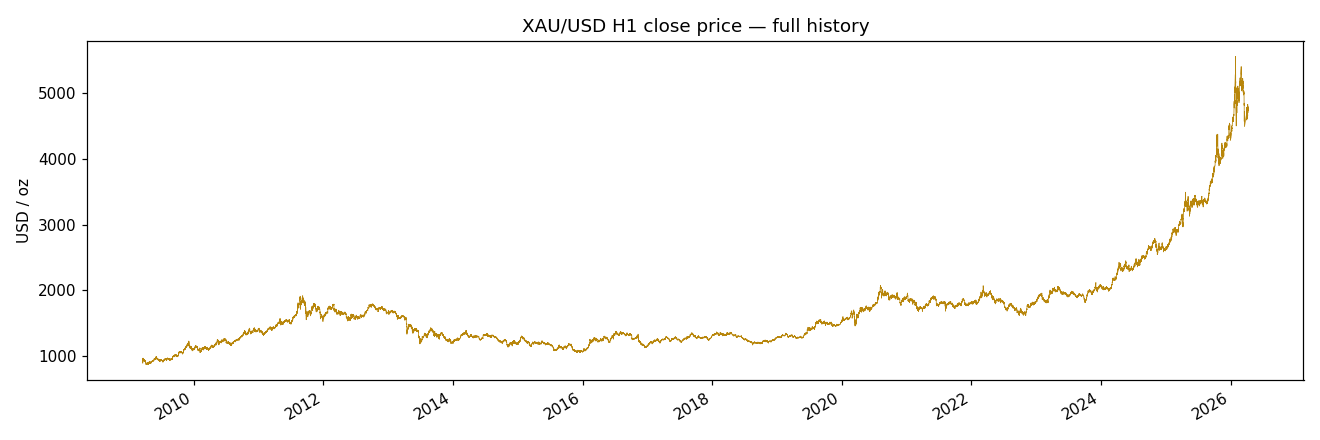
\includegraphics[width=\linewidth]{01_price_history.png}
\caption{Historique du prix de clôture XAU/USD en H1 (2009--2026).}
\end{figure}
\noindent\textbf{Interprétation.} La série couvre 17 ans (101\,334 bougies). On
distingue nettement plusieurs régimes : la consolidation post-crise (2011--2015),
le rebond 2019--2020, puis surtout la forte tendance haussière 2023--2026 où l'or
passe d'environ 1\,900\,\$ à 4\,760\,\$ (+150\,\%). Cette rupture de régime entre
la période d'entraînement (2009--2020) et de test (2023--2026) est l'élément
explicatif central de tous les résultats : un modèle appris sur l'ancien régime
généralise mal sur le nouveau.

\begin{figure}[H]
\centering
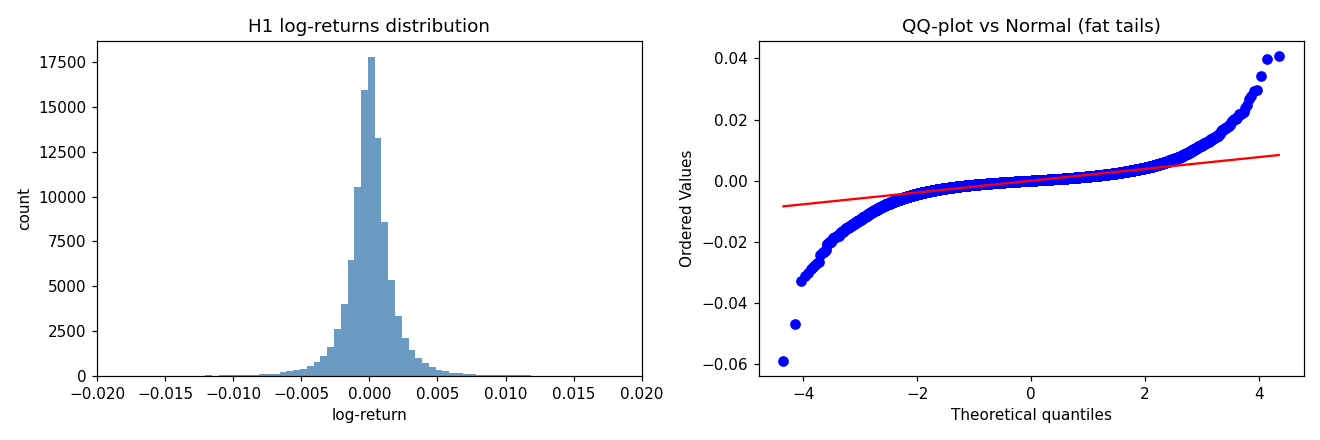
\includegraphics[width=\linewidth]{02_returns_distribution.png}
\caption{Distribution des log-rendements H1 (gauche) et QQ-plot vs loi normale (droite).}
\end{figure}
\noindent\textbf{Interprétation.} La distribution des rendements est fortement
leptokurtique (kurtosis $\approx 27.9$) et légèrement asymétrique à gauche
(skewness $\approx -0.47$). Le QQ-plot s'écarte massivement de la droite normale
aux extrémités : les queues sont beaucoup plus épaisses qu'une gaussienne
(\emph{fat tails}). Conséquence méthodologique : les pertes quadratiques (RMSE)
sont dominées par quelques mouvements extrêmes, ce qui justifie de compléter
l'évaluation par des métriques directionnelles et un ratio de Sharpe.

\begin{figure}[H]
\centering
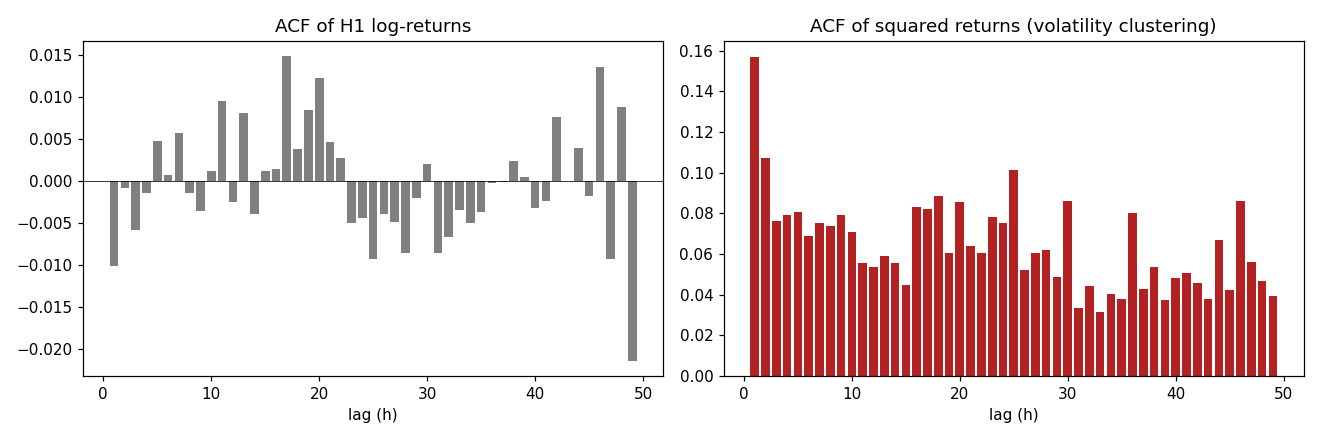
\includegraphics[width=\linewidth]{03_volatility_clustering.png}
\caption{Autocorrélation des rendements (gauche) et des rendements au carré (droite).}
\end{figure}
\noindent\textbf{Interprétation.} L'ACF des rendements est quasi nulle à tous les
retards : les rendements eux-mêmes sont proches d'un bruit blanc (cohérent avec
l'efficience faible du marché). En revanche, l'ACF des rendements au carré est
positive et décroît lentement : c'est la signature classique du
\emph{volatility clustering} (les périodes de forte volatilité se regroupent).
Cela motive l'usage de la volatilité réalisée comme feature et comme seuil
adaptatif pour la cible de classification.

\begin{figure}[H]
\centering
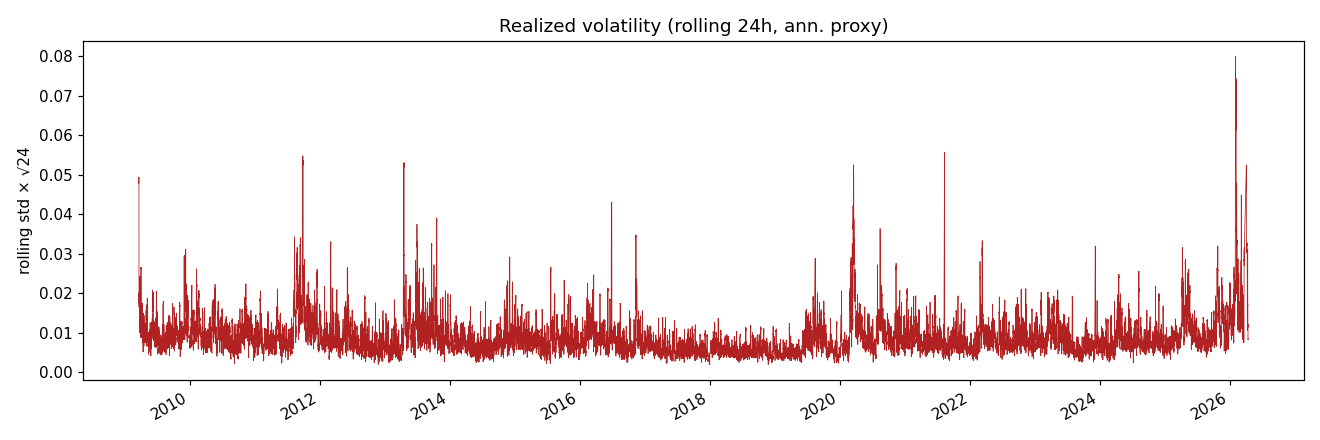
\includegraphics[width=\linewidth]{04_realized_volatility.png}
\caption{Volatilité réalisée glissante 24h (annualisée approx.).}
\end{figure}
\noindent\textbf{Interprétation.} La volatilité n'est pas stationnaire : pics
marqués lors des chocs (2020, 2022, 2024). Ce caractère hétéroscédastique
confirme la pertinence d'un seuil de zone neutre proportionnel à la volatilité
passée plutôt qu'un seuil fixe.

\begin{figure}[H]
\centering
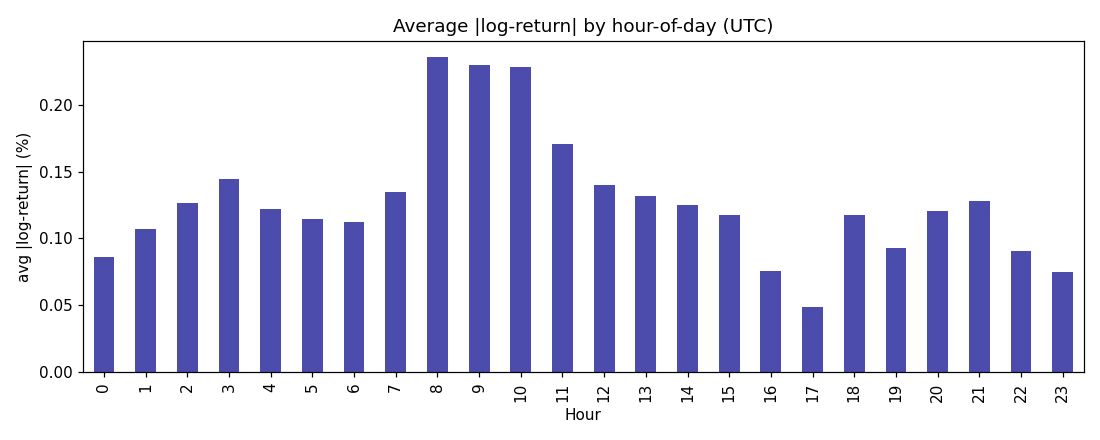
\includegraphics[width=\linewidth]{05_intraday_seasonality.png}
\caption{Amplitude moyenne des rendements absolus par heure (UTC).}
\end{figure}
\noindent\textbf{Interprétation.} La saisonnalité intra-journalière montre une
amplitude accrue lors du recouvrement des sessions de Londres et de New York
(après-midi UTC), et plus faible la nuit (session asiatique). Cette structure
justifie les features calendaires (encodage sin/cos de l'heure et indicateurs de
session) et confirme que le fuseau retenu (UTC) est cohérent.

% =====================================================================
\section{Phase 2 — Features et cibles}
% =====================================================================

\begin{figure}[H]
\centering
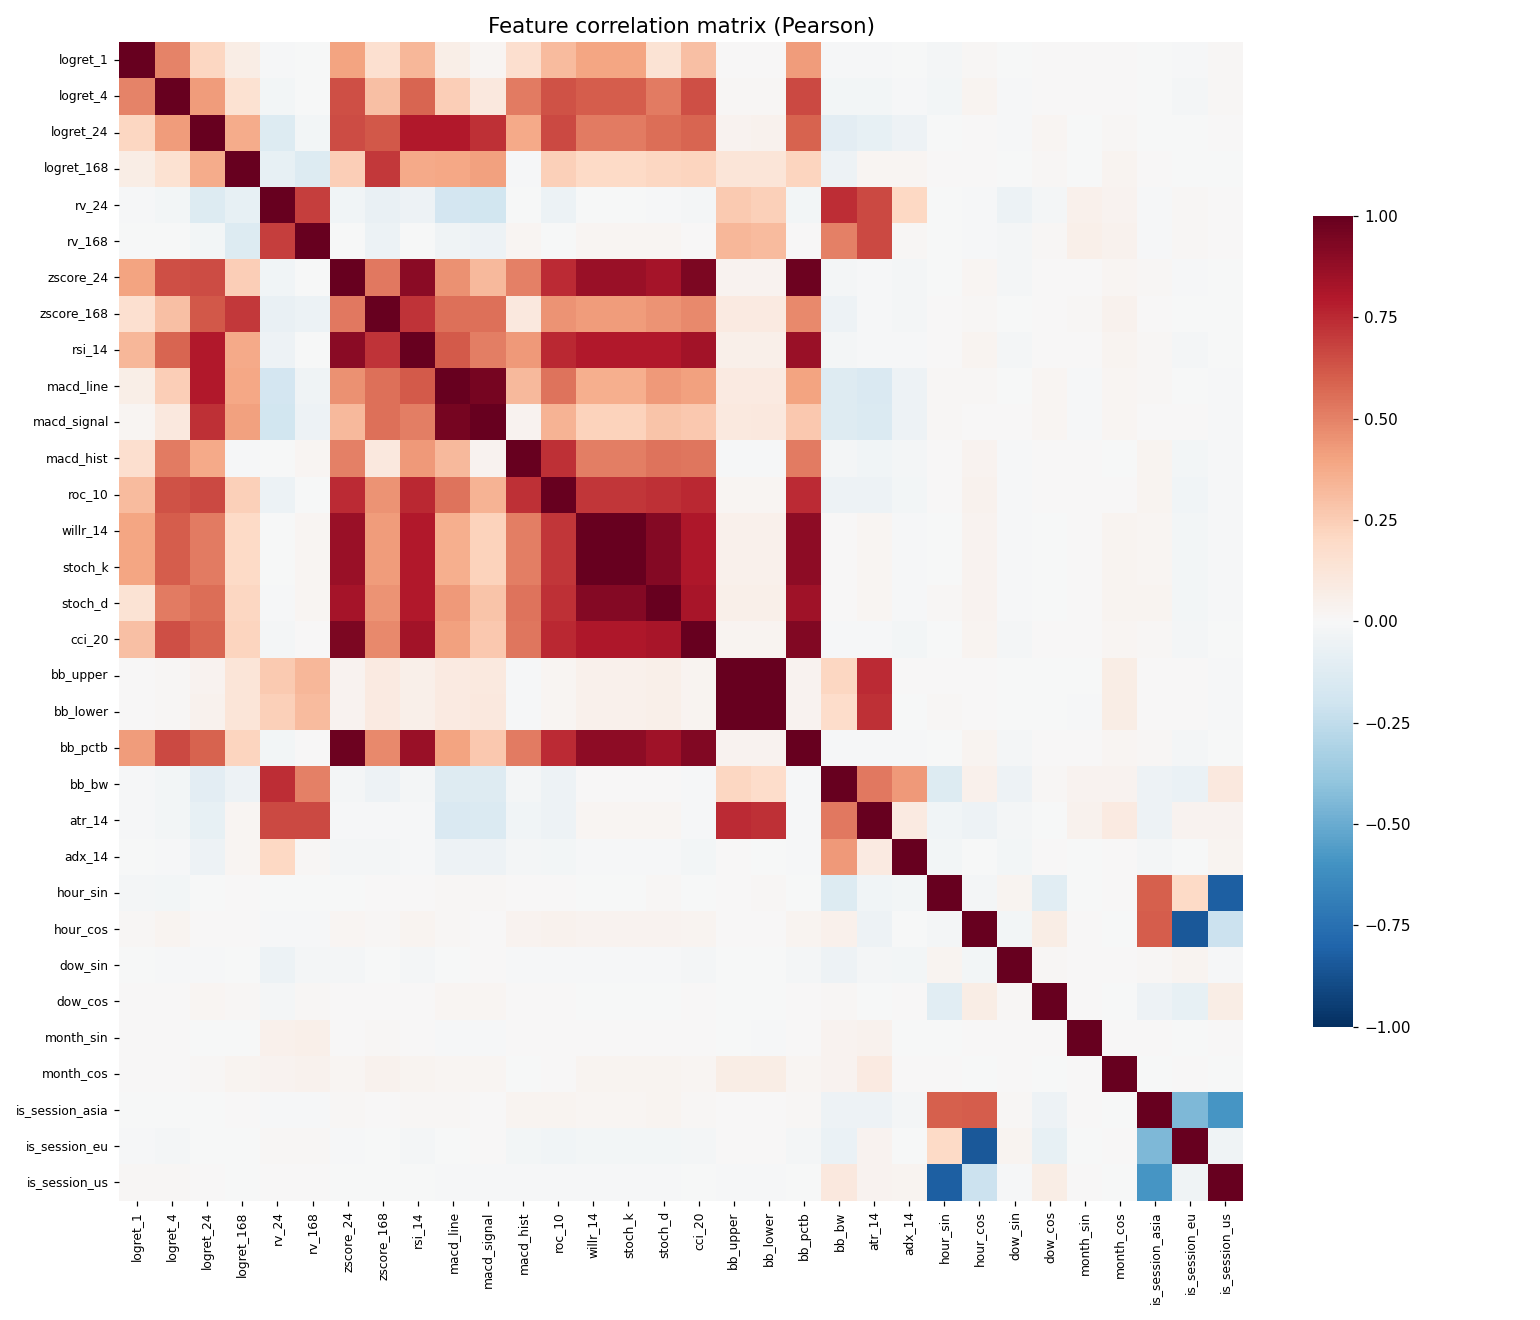
\includegraphics[width=0.85\linewidth]{06_feature_correlation.png}
\caption{Matrice de corrélation de Pearson des 62 features.}
\end{figure}
\noindent\textbf{Interprétation.} On observe des blocs de forte corrélation
attendus : indicateurs de tendance entre eux (MACD, ROC), bandes de Bollinger
avec le niveau de prix, mesures de volatilité (ATR, RV24, RV168). Ces redondances
ne nuisent pas aux modèles à arbres (robustes à la colinéarité) mais justifient
la standardisation pour les modèles linéaires/DL.

\begin{figure}[H]
\centering
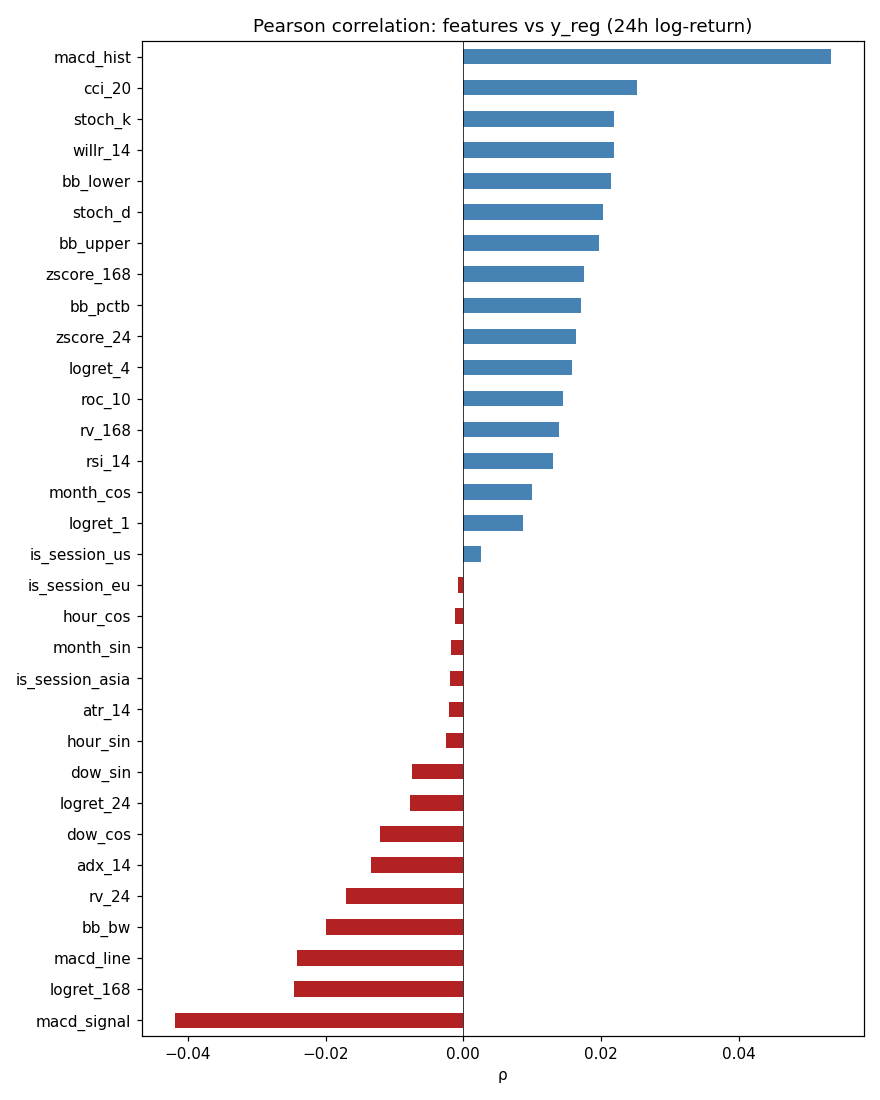
\includegraphics[width=0.7\linewidth]{07_feature_target_corr.png}
\caption{Corrélation de Pearson de chaque feature avec la cible $y_{reg}$.}
\end{figure}
\noindent\textbf{Interprétation.} Aucune feature ne dépasse $|\rho|\approx 0.05$
avec la cible. C'est un résultat fondamental : à horizon 24h, \emph{aucune
variable seule n'a de pouvoir prédictif linéaire significatif}. Cela borne par
avance la performance atteignable et explique les $R^2$ négatifs observés ensuite.

\begin{figure}[H]
\centering
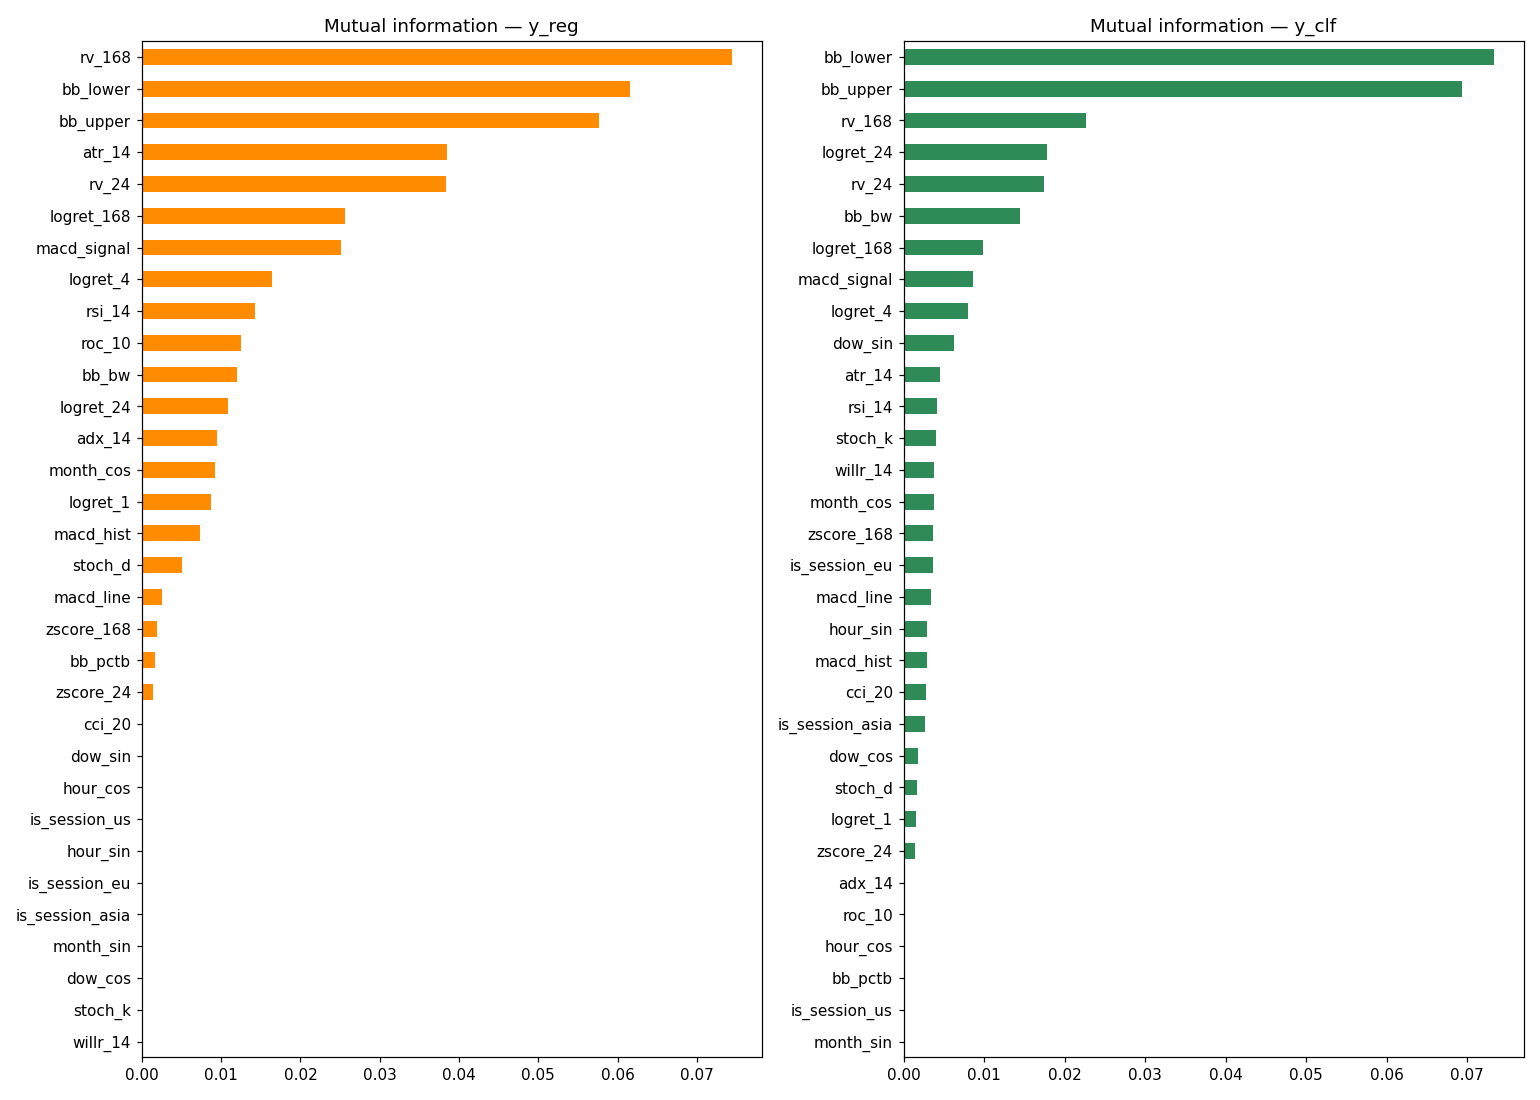
\includegraphics[width=\linewidth]{08_mutual_information.png}
\caption{Information mutuelle des features avec $y_{reg}$ (gauche) et $y_{clf}$ (droite).}
\end{figure}
\noindent\textbf{Interprétation.} L'information mutuelle (qui capte aussi les
dépendances non linéaires) classe en tête les features de volatilité
(\texttt{rv\_168}, \texttt{atr\_14}, bandes de Bollinger). Le signal exploitable
est donc davantage lié à l'\emph{amplitude} future qu'à la \emph{direction} —
cohérent avec le volatility clustering et avec la difficulté de prédire le signe.

\begin{figure}[H]
\centering
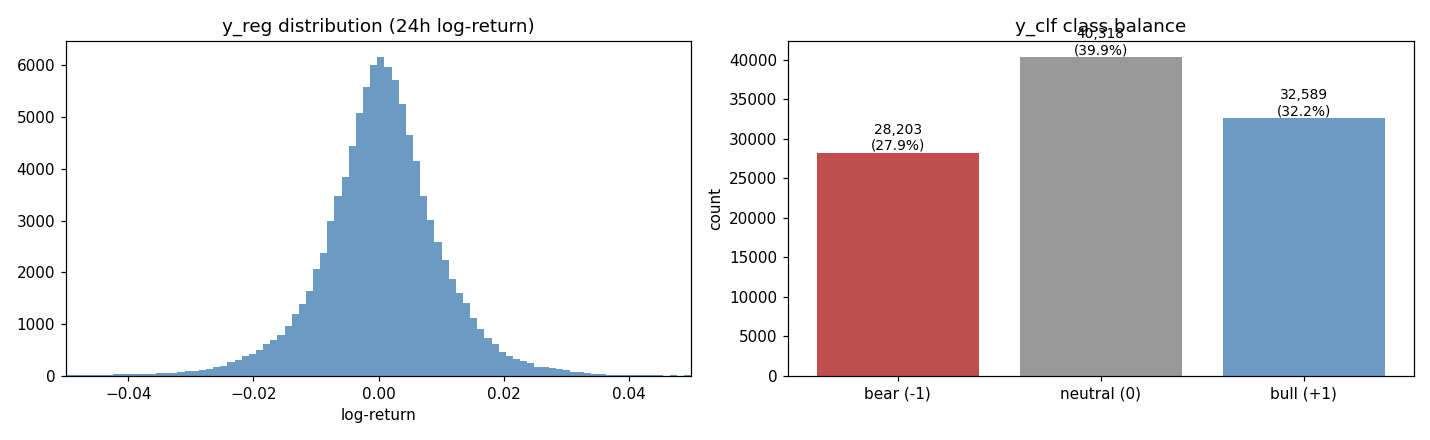
\includegraphics[width=\linewidth]{09_target_distribution.png}
\caption{Distribution de $y_{reg}$ (gauche) et équilibre des classes $y_{clf}$ (droite).}
\end{figure}
\noindent\textbf{Interprétation.} La cible de régression est centrée, leptokurtique.
La cible ternaire est raisonnablement équilibrée (39.9\,\% neutre, 32.2\,\% hausse,
27.9\,\% baisse) grâce au seuil adaptatif $0.5\,\sigma\sqrt{h}$, ce qui évite un
classifieur trivial et rend la métrique MCC informative.

% =====================================================================
\section{Phase 4 — Modèles individuels (horizon h=24, statique)}
% =====================================================================

\subsection{XGBoost}
\begin{figure}[H]
\centering
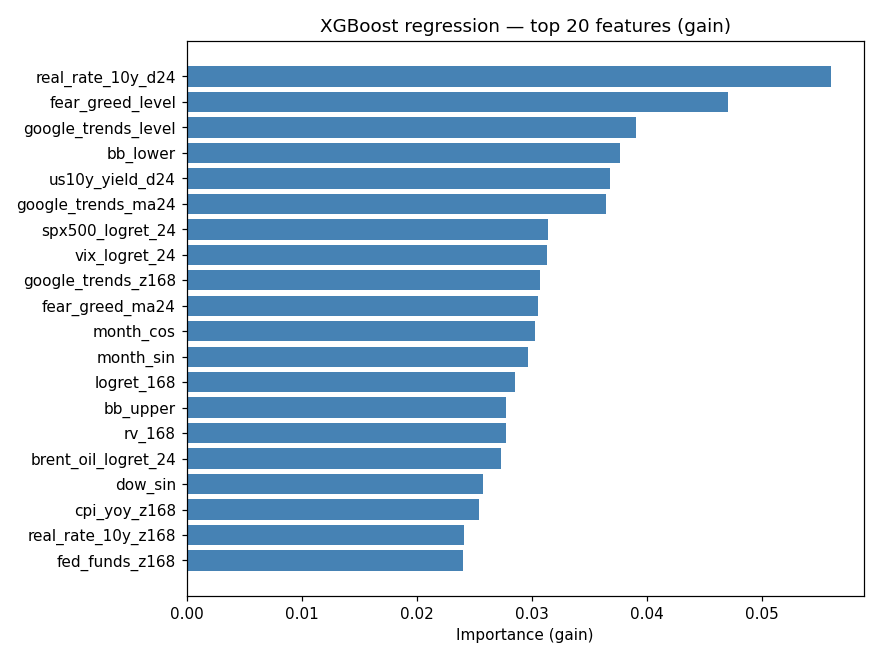
\includegraphics[width=0.7\linewidth]{xgboost/xgb_regression_feature_importance.png}
\caption{Importance des features (gain) — XGBoost régression.}
\end{figure}
\noindent\textbf{Interprétation.} Les features dominantes sont liées à la
volatilité et aux niveaux de Bollinger, confirmant l'analyse d'information
mutuelle. Le modèle s'appuie donc surtout sur l'état de volatilité, peu sur un
signal directionnel.

\begin{figure}[H]
\centering
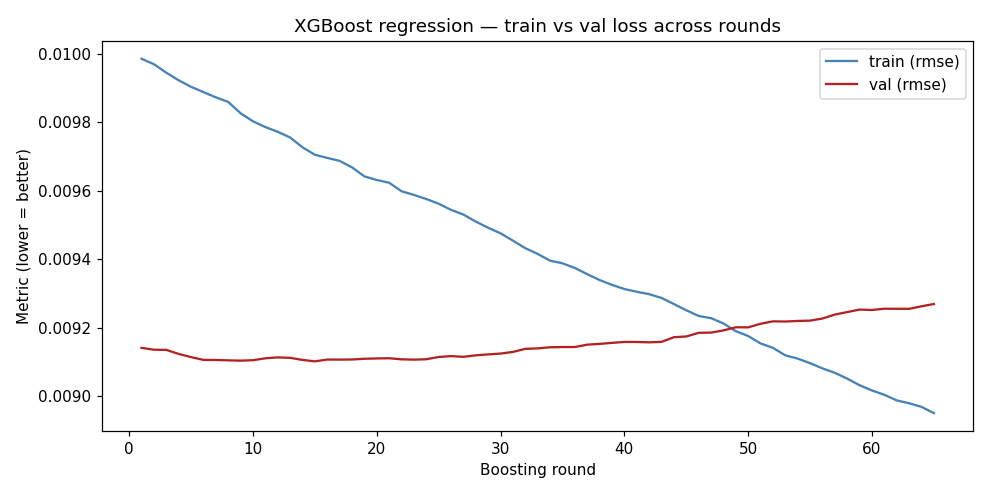
\includegraphics[width=0.95\linewidth]{xgboost/xgb_regression_loss_curve.png}
\caption{Courbe de perte train vs validation par itération de boosting — XGBoost.}
\end{figure}
\noindent\textbf{Interprétation.} La perte d'entraînement décroît régulièrement
tandis que la perte de validation plafonne puis stagne : c'est le signe d'un
apprentissage qui n'apporte plus de gain de généralisation au-delà des premières
centaines d'arbres. L'early stopping est donc justifié.

\begin{figure}[H]
\centering
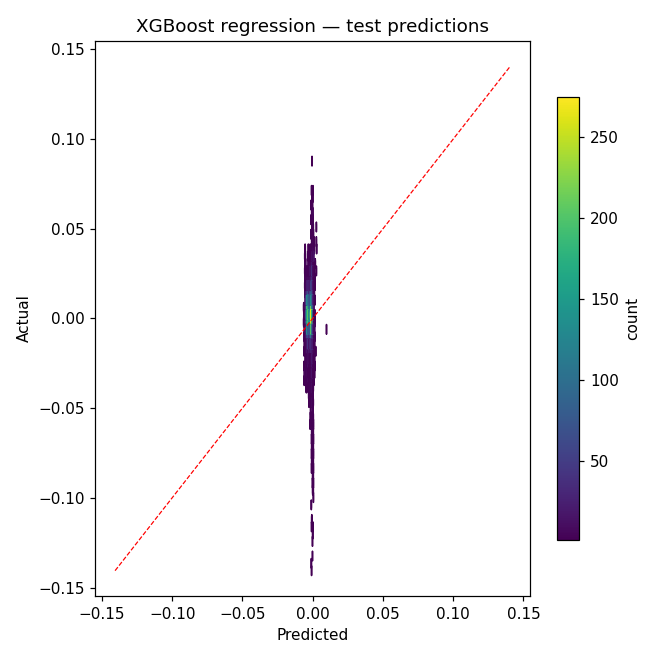
\includegraphics[width=0.55\linewidth]{xgboost/xgb_reg_pred_vs_actual.png}
\hfill
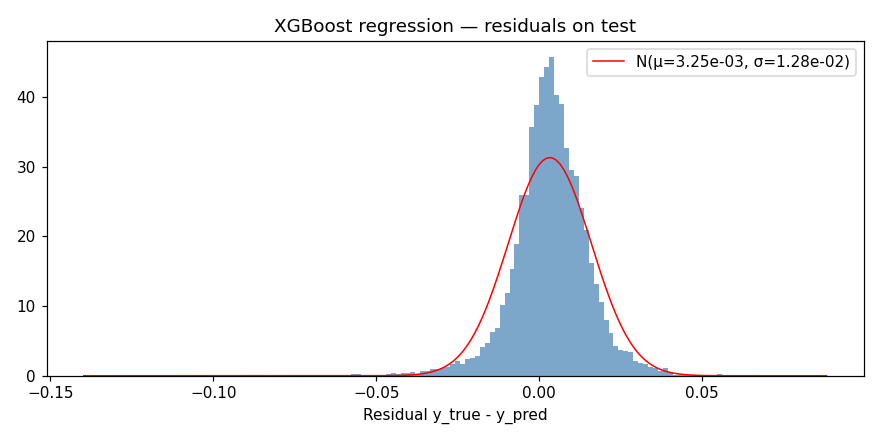
\includegraphics[width=0.42\linewidth]{xgboost/xgb_reg_residuals.png}
\caption{Predicted vs actual (gauche) et distribution des résidus (droite) — XGBoost test.}
\end{figure}
\noindent\textbf{Interprétation.} Le nuage predicted/actual est quasi vertical :
le modèle prédit des valeurs de faible amplitude (proches de zéro) quelle que
soit la réalité, traduisant l'absence de pouvoir prédictif en niveau ($R^2=-0.08$).
Les résidus restent centrés mais à variance élevée.

\begin{figure}[H]
\centering
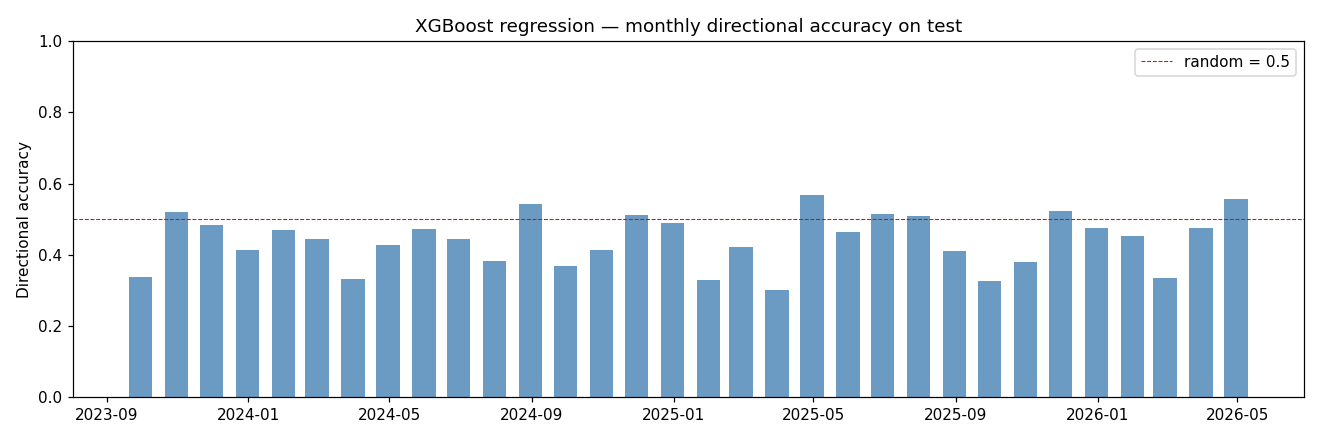
\includegraphics[width=0.95\linewidth]{xgboost/xgb_reg_monthly_dir_acc.png}
\caption{Précision directionnelle mensuelle sur le test — XGBoost.}
\end{figure}
\noindent\textbf{Interprétation.} La précision directionnelle oscille fortement
autour de 0,5 selon les mois, sans biais positif stable. Le modèle n'extrait pas
de signal directionnel robuste sur la période de test.

\paragraph{Classification XGBoost.}
\begin{figure}[H]
\centering
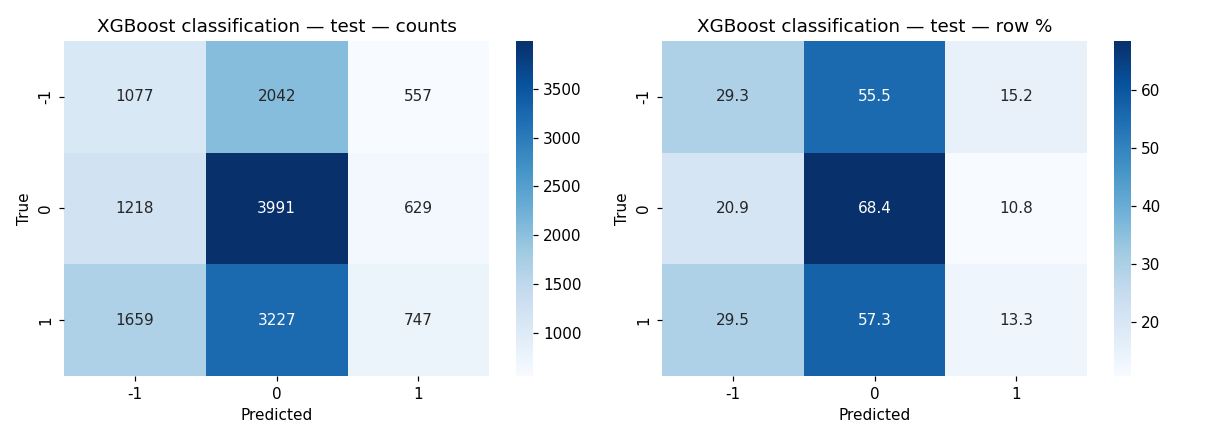
\includegraphics[width=0.48\linewidth]{xgboost/xgb_clf_confusion.png}
\hfill
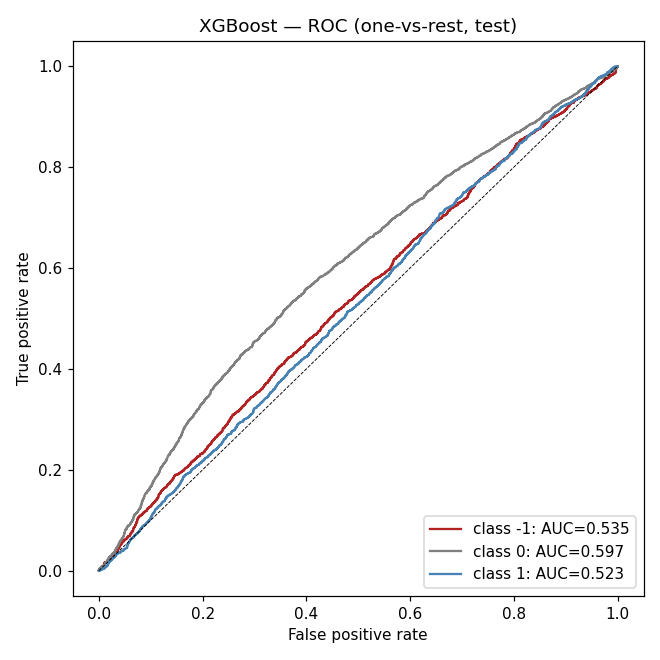
\includegraphics[width=0.48\linewidth]{xgboost/xgb_clf_roc.png}
\caption{Matrice de confusion (gauche) et courbes ROC one-vs-rest (droite) — XGBoost classification.}
\end{figure}
\noindent\textbf{Interprétation.} En classification ternaire, XGBoost dépasse
légèrement le baseline majoritaire (MCC$\approx 0.06>0$), les AUC ROC restant
proches de 0,5--0,55. Le ternarisation par seuil de volatilité rend la tâche un
peu plus apprenable que la régression pure, sans pour autant fournir un signal
fort. Les courbes Precision-Recall (\texttt{xgb\_clf\_pr.png}) et le rapport de
classification (\texttt{xgb\_clf\_report.png}) confirment des performances par
classe modestes mais supérieures au hasard.

\subsection{Random Forest}
\begin{figure}[H]
\centering
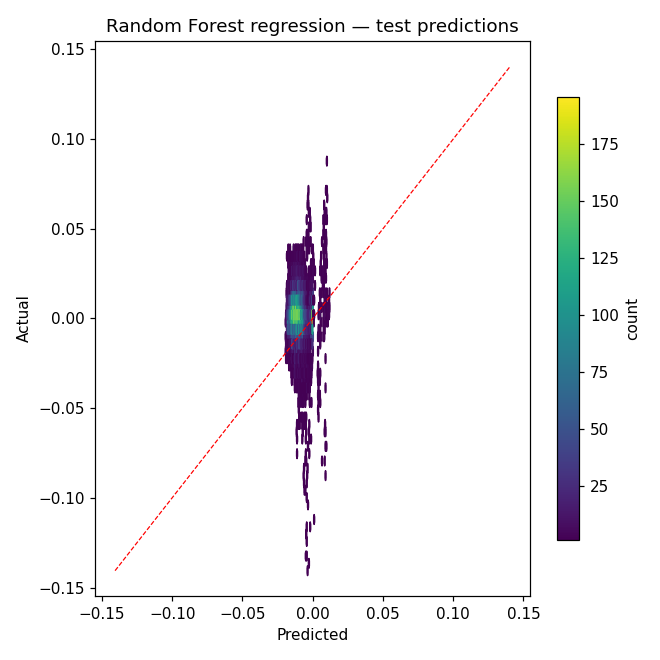
\includegraphics[width=0.55\linewidth]{random_forest/rf_reg_pred_vs_actual.png}
\hfill
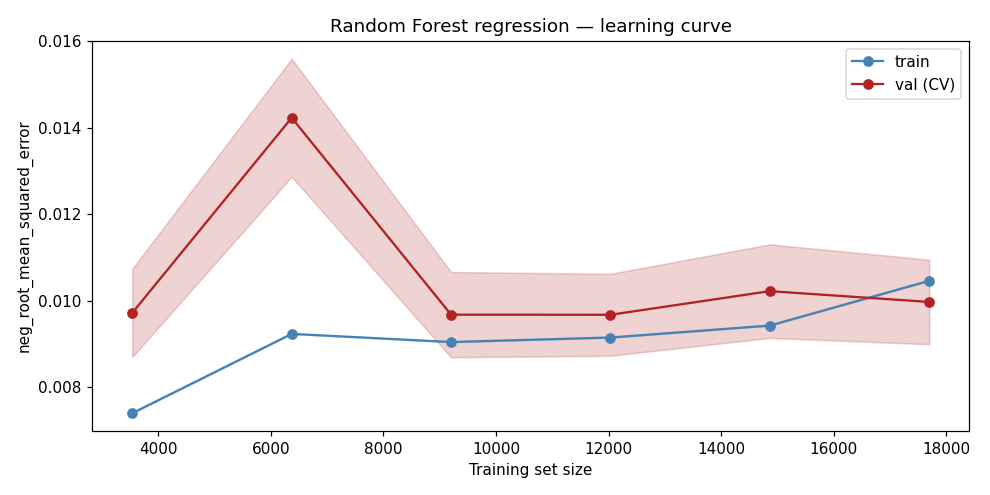
\includegraphics[width=0.42\linewidth]{random_forest/rf_reg_learning_curve.png}
\caption{Predicted vs actual (gauche) et learning curve (droite) — Random Forest régression.}
\end{figure}
\noindent\textbf{Interprétation.} Random Forest présente le pire $R^2$ test
($-0.96$) parmi les modèles à arbres. La learning curve (perte vs taille du train
en validation croisée temporelle) montre un écart persistant train/validation :
le modèle mémorise le train sans transférer. C'est l'illustration que sur données
financières non stationnaires, augmenter la capacité aggrave le surapprentissage.

\begin{figure}[H]
\centering
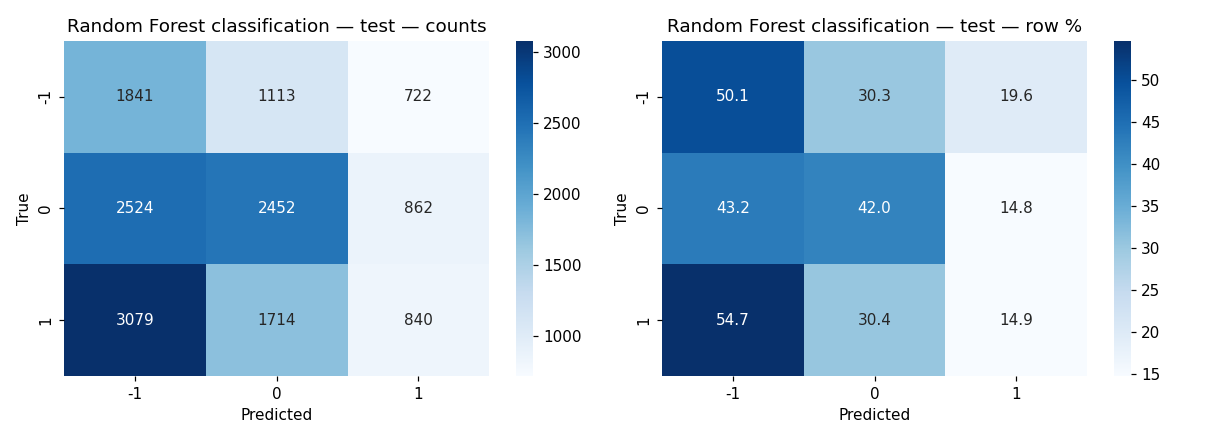
\includegraphics[width=0.48\linewidth]{random_forest/rf_clf_confusion.png}
\hfill
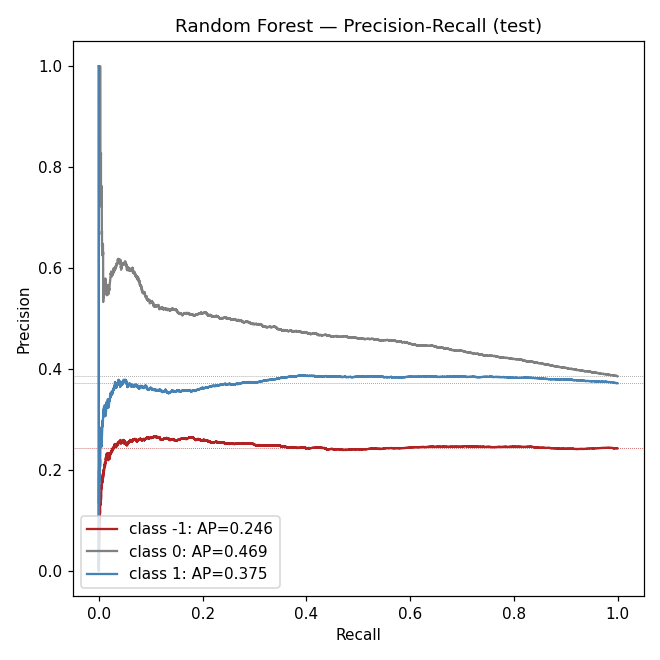
\includegraphics[width=0.48\linewidth]{random_forest/rf_clf_pr.png}
\caption{Confusion (gauche) et Precision-Recall (droite) — Random Forest classification.}
\end{figure}
\noindent\textbf{Interprétation.} En classification, le train atteint un MCC très
élevé (mémorisation, \texttt{max\_depth} profond) qui ne se transfère pas au test
(MCC$\approx 0.04$). Le diagnostic d'overfit est sans ambiguïté.

\subsection{CNN 1D et BiGRU (Deep Learning)}
\begin{figure}[H]
\centering
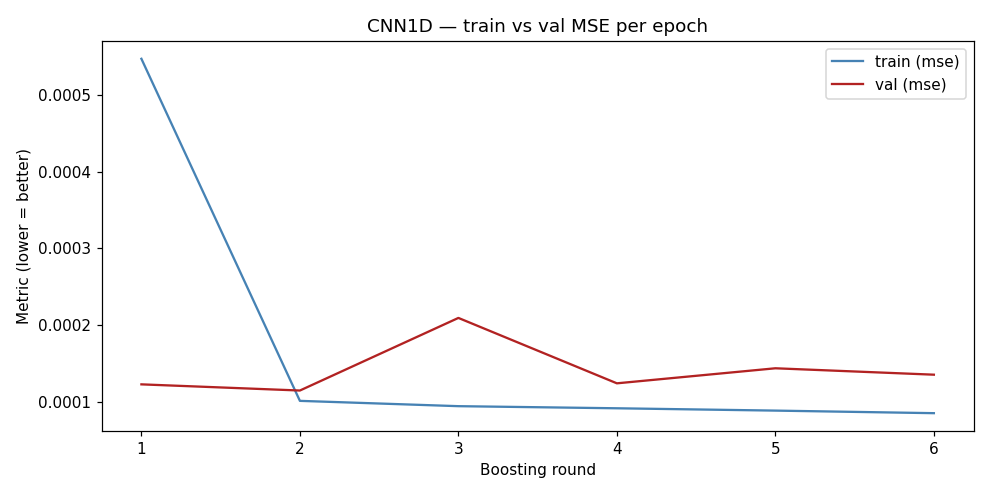
\includegraphics[width=0.48\linewidth]{cnn/cnn_reg_loss_curve.png}
\hfill
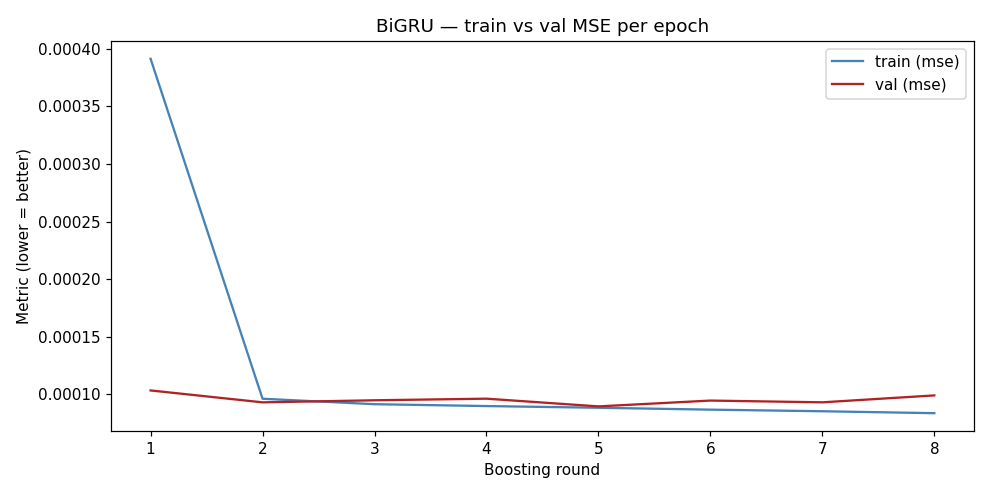
\includegraphics[width=0.48\linewidth]{bigru/bigru_reg_loss_curve.png}
\caption{Courbes de perte MSE train vs val — CNN 1D (gauche) et BiGRU (droite).}
\end{figure}
\noindent\textbf{Interprétation.} Les deux réseaux convergent proprement sur
train et val, mais l'early stopping se déclenche tôt (la val ne progresse plus).
Ils obtiennent les pires $R^2$ test ($-2.08$ et $-1.83$) : plus le modèle est
flexible, plus il s'ajuste à des motifs du régime 2009--2020 qui s'inversent en
2023--2026.

\begin{figure}[H]
\centering
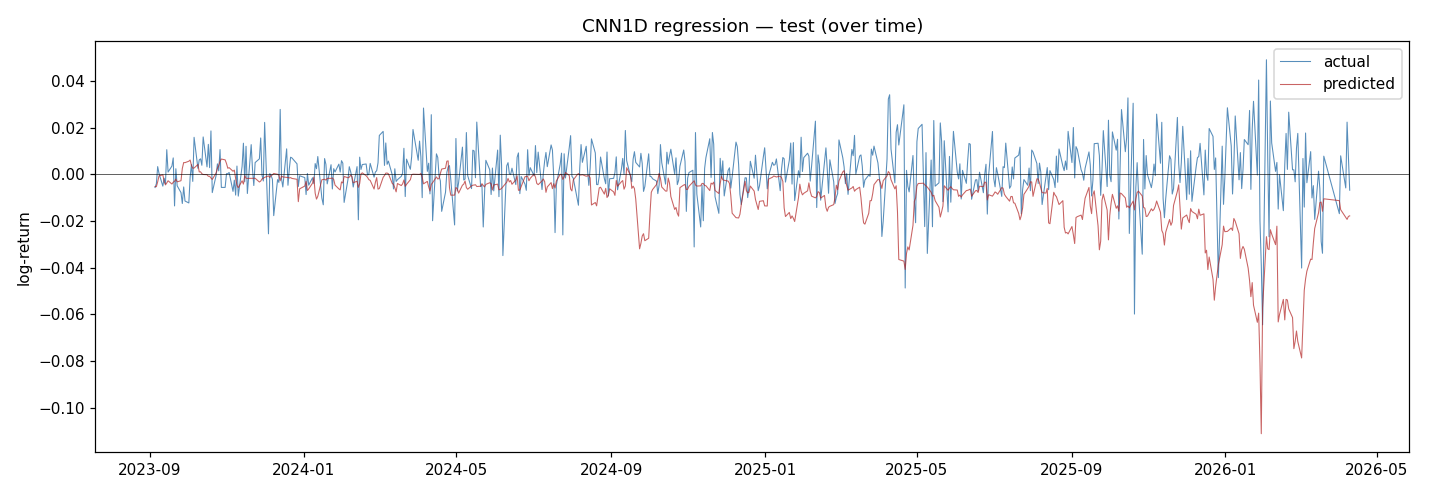
\includegraphics[width=0.48\linewidth]{cnn/cnn_reg_pred_vs_actual_ts.png}
\hfill
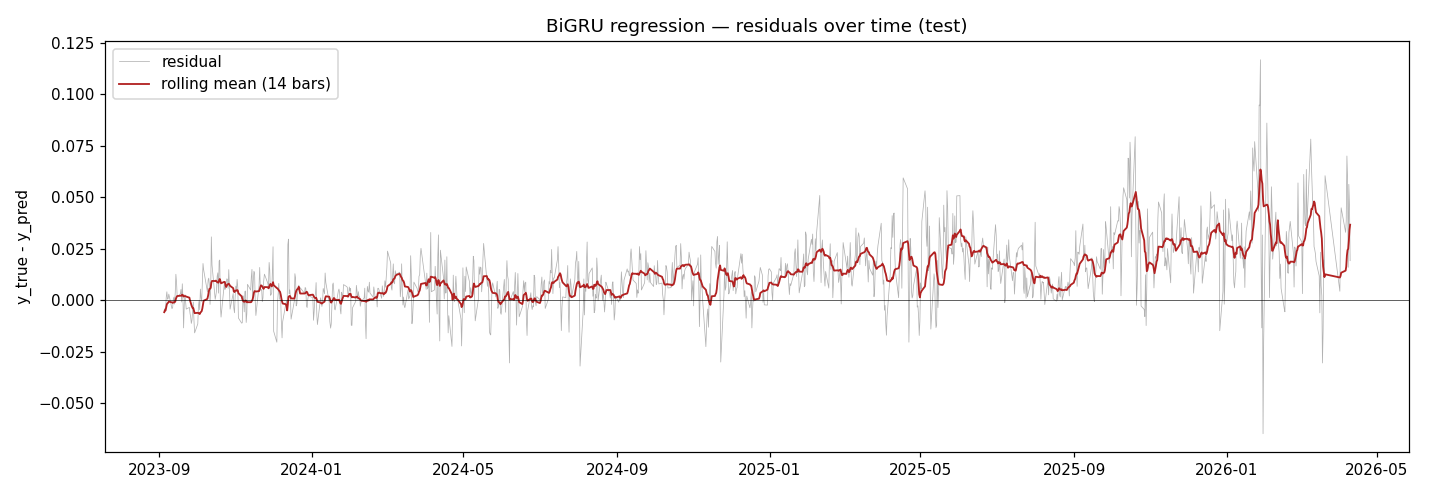
\includegraphics[width=0.48\linewidth]{bigru/bigru_reg_residuals_over_time.png}
\caption{Prédiction vs réel dans le temps — CNN (gauche) ; résidus dans le temps — BiGRU (droite).}
\end{figure}
\noindent\textbf{Interprétation.} La série prédite par le CNN reste collée près
de zéro tandis que le réel oscille fortement : le réseau a appris la moyenne du
train. Les résidus du BiGRU dérivent négativement après mi-2024 (biais $\approx
-1.3\,\%$) : le modèle sous-estime systématiquement la hausse de l'or sur la
période récente.

% =====================================================================
\section{Phase 5 — Comparaison inter-modèles (h=24 statique)}
% =====================================================================

\begin{figure}[H]
\centering
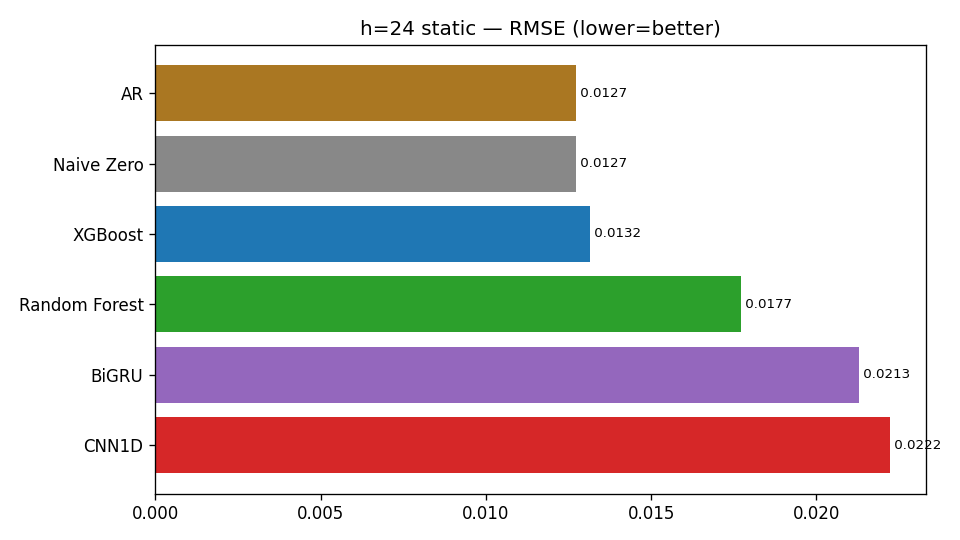
\includegraphics[width=0.49\linewidth]{comparison/cmp_h24_rmse.png}
\hfill
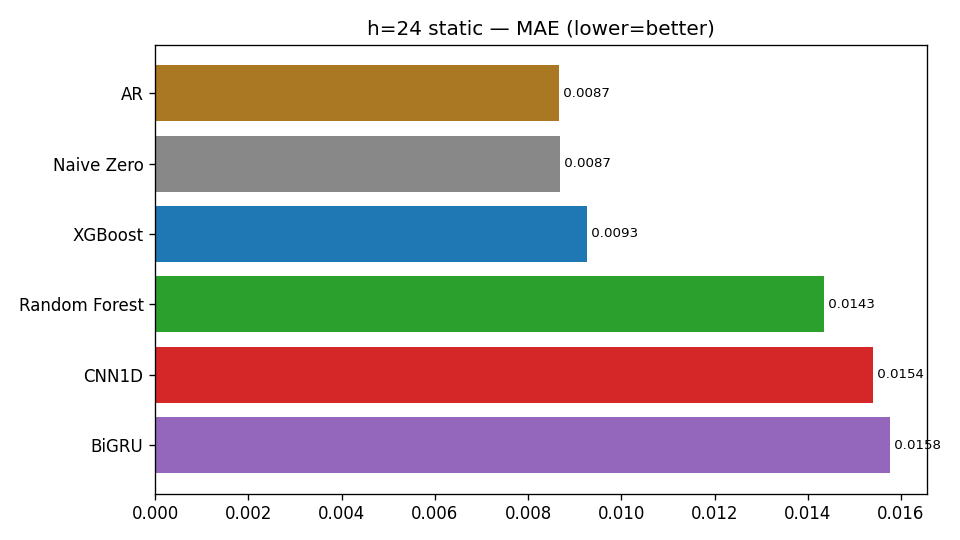
\includegraphics[width=0.49\linewidth]{comparison/cmp_h24_mae.png}
\caption{RMSE (gauche) et MAE (droite) par modèle — test h=24.}
\end{figure}
\noindent\textbf{Interprétation.} Le baseline naïf (prédiction nulle) et l'AR
réalisent les meilleures RMSE/MAE ; tous les modèles ML/DL font \emph{moins bien}.
C'est contre-intuitif mais cohérent : prédire zéro est optimal sous l'hypothèse de
martingale, et les modèles complexes ajoutent du bruit.

\begin{figure}[H]
\centering
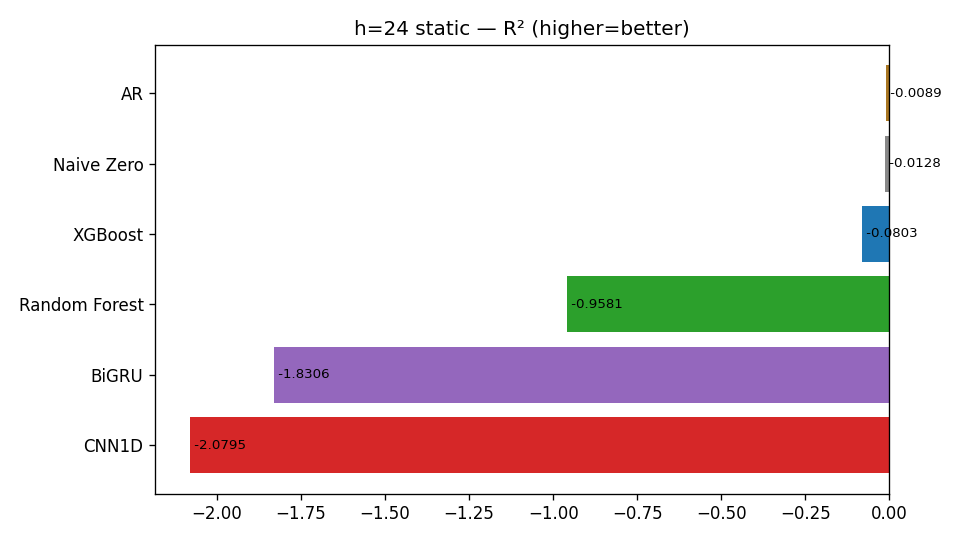
\includegraphics[width=0.49\linewidth]{comparison/cmp_h24_r2.png}
\hfill
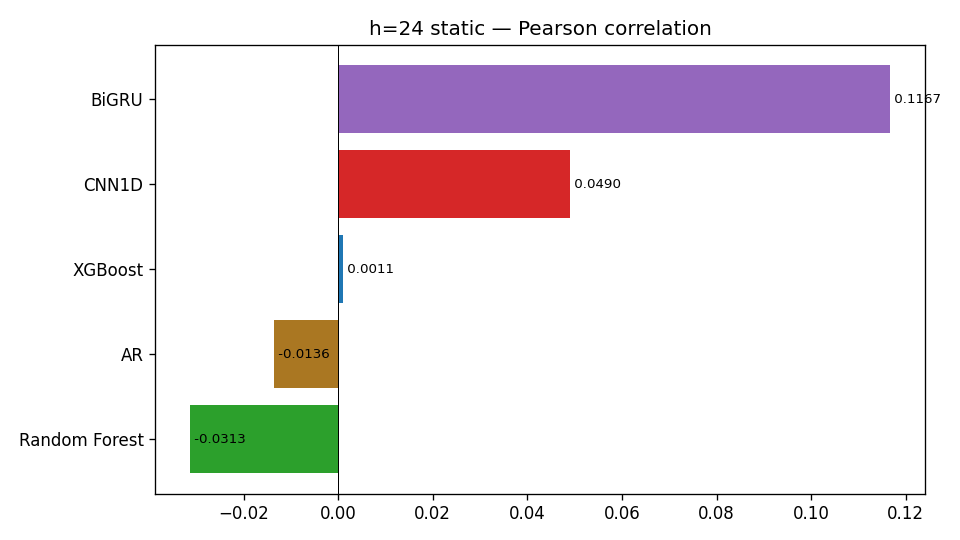
\includegraphics[width=0.49\linewidth]{comparison/cmp_h24_pearson.png}
\caption{$R^2$ (gauche) et corrélation de Pearson (droite) par modèle — test h=24.}
\end{figure}
\noindent\textbf{Interprétation.} Tous les $R^2$ test sont négatifs, et d'autant
plus négatifs que le modèle est complexe (Naïve $\approx 0 >$ XGBoost $>$ RF $>$
BiGRU $>$ CNN). La corrélation de Pearson reste proche de zéro pour tous. Conclusion
claire : à h=24, la prédiction \emph{en niveau} du rendement est hors de portée.

\begin{figure}[H]
\centering
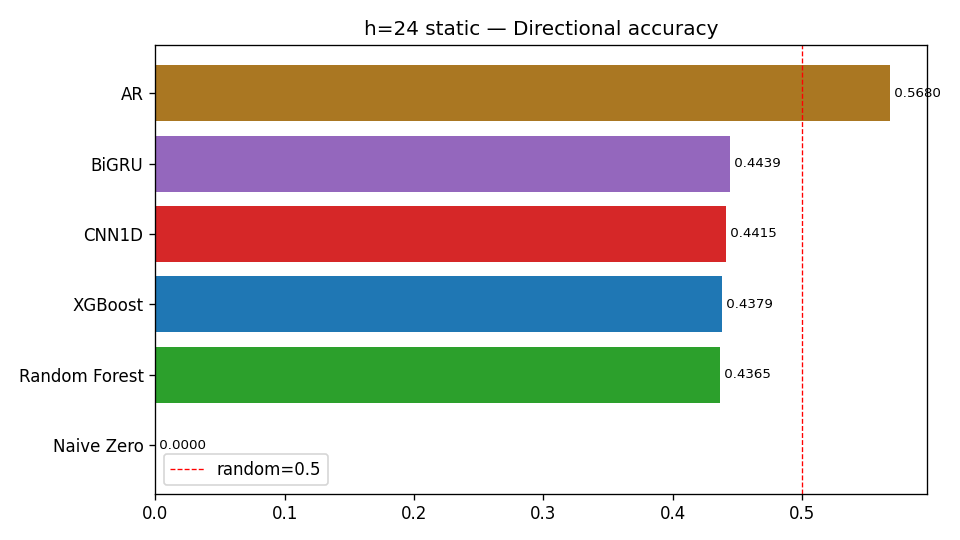
\includegraphics[width=0.7\linewidth]{comparison/cmp_h24_directional_accuracy.png}
\caption{Précision directionnelle par modèle — test h=24 (ligne rouge = hasard).}
\end{figure}
\noindent\textbf{Interprétation.} Aucun modèle entraîné ne dépasse nettement
0,5. Seuls l'AR (par construction momentum) et le TSFM Chronos affichent une
précision marginalement supérieure. La direction à h=24 n'est pas exploitable de
façon fiable.

\begin{figure}[H]
\centering
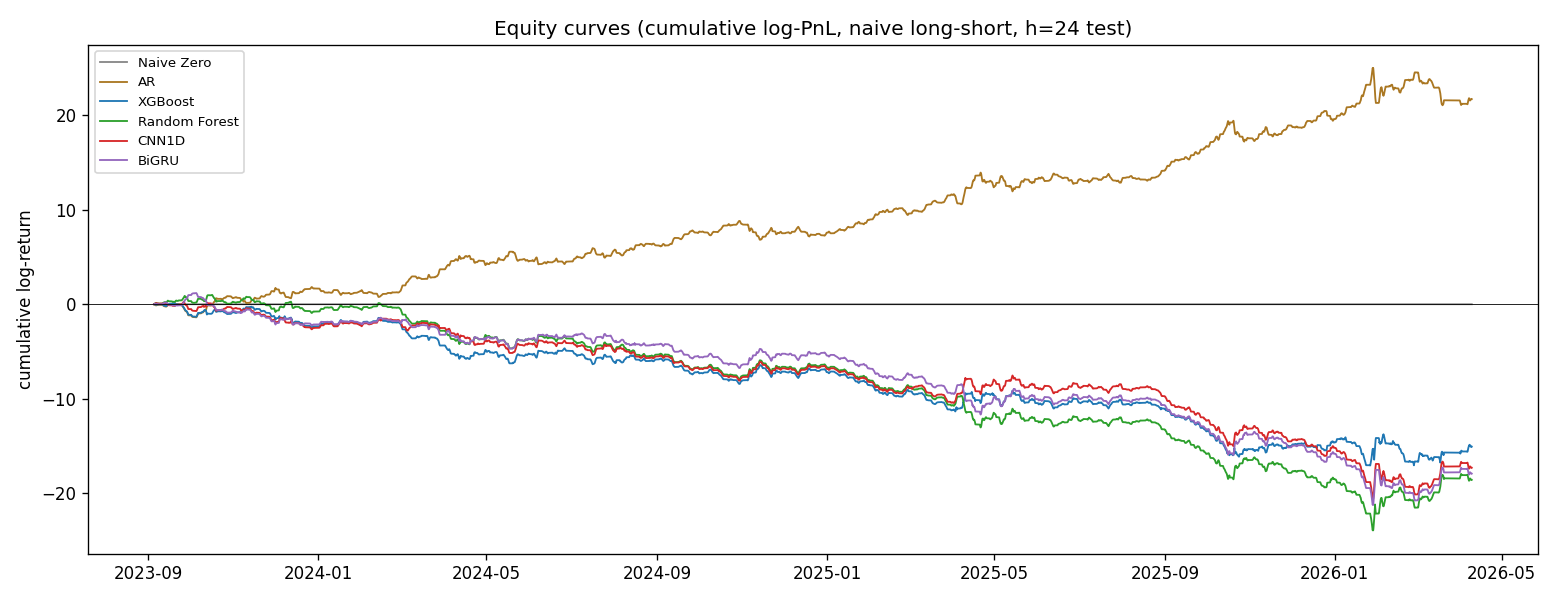
\includegraphics[width=\linewidth]{comparison/cmp_h24_equity_curves.png}
\caption{Courbes d'equity (PnL log cumulé d'une stratégie long-short naïve) — test h=24.}
\end{figure}
\noindent\textbf{Interprétation.} Aucune courbe d'equity ne présente de tendance
haussière franche et régulière : les stratégies dérivées des prédictions h=24
n'auraient pas été profitables. C'est la traduction « trading » des $R^2$ négatifs.

\begin{figure}[H]
\centering
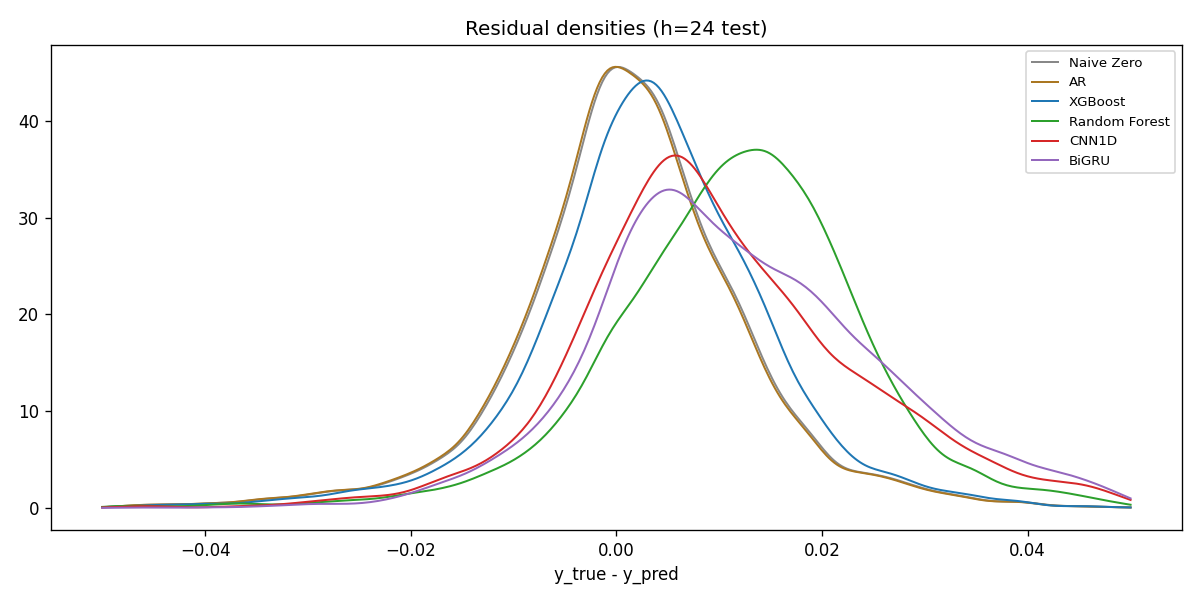
\includegraphics[width=0.49\linewidth]{comparison/cmp_h24_residual_kde.png}
\hfill
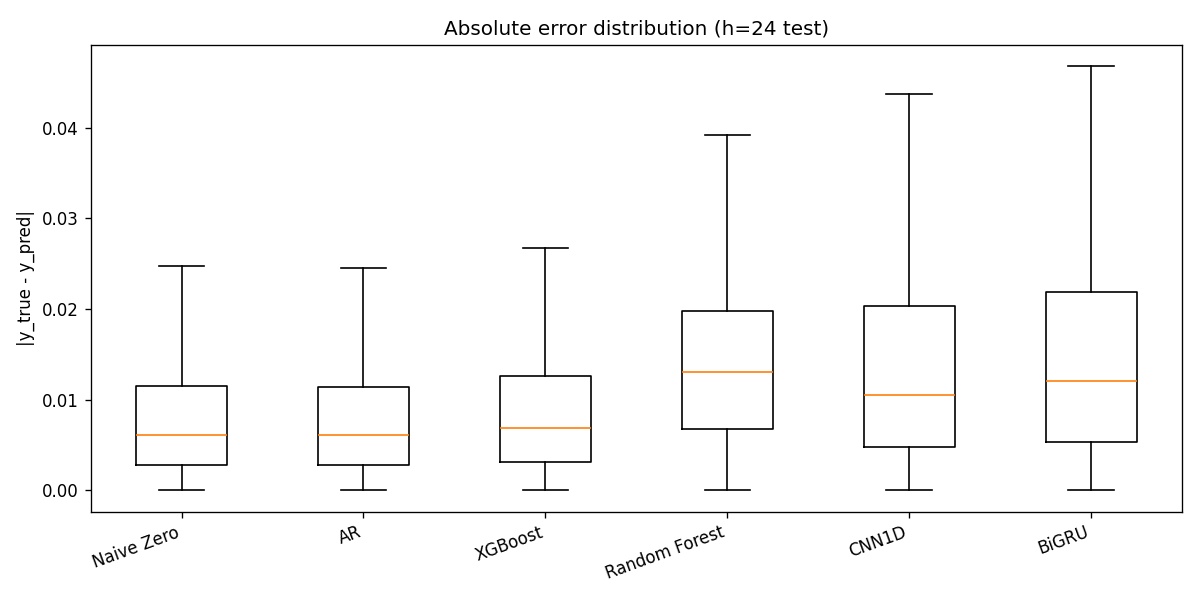
\includegraphics[width=0.49\linewidth]{comparison/cmp_h24_abs_error_box.png}
\caption{Densités de résidus (gauche) et boxplots d'erreur absolue (droite) — test h=24.}
\end{figure}
\noindent\textbf{Interprétation.} Naïve et AR ont les densités de résidus les
plus resserrées ; les modèles DL ont des résidus plus dispersés (erreurs plus
grandes), confirmant la hiérarchie des RMSE.

\begin{figure}[H]
\centering
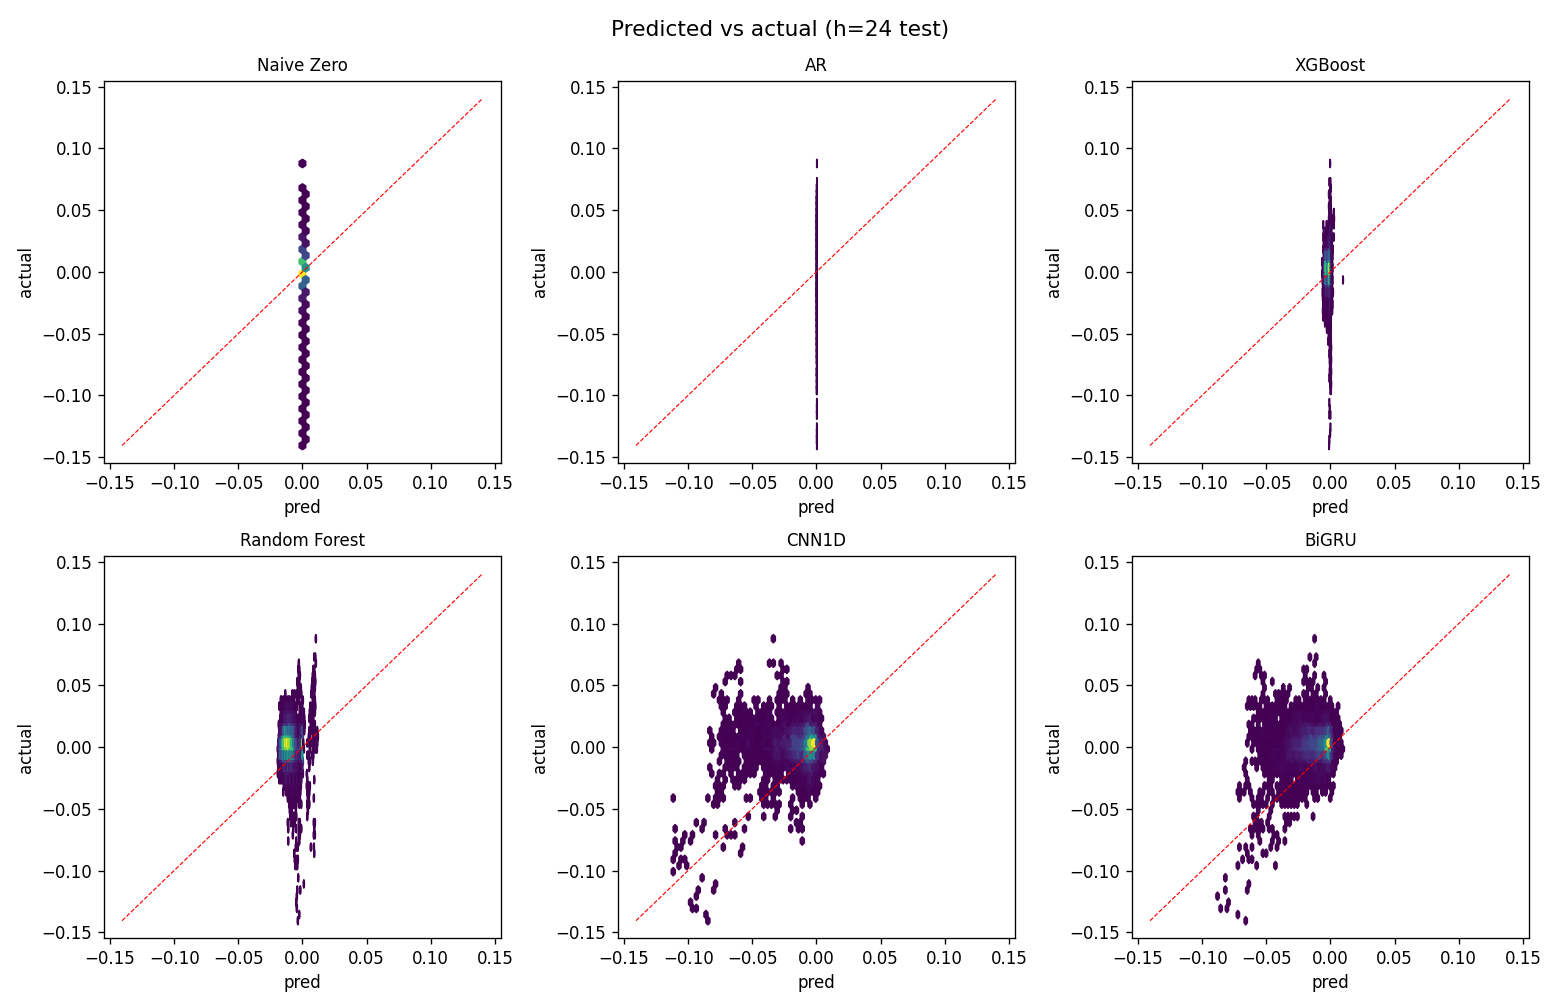
\includegraphics[width=\linewidth]{comparison/cmp_h24_pred_vs_actual_grid.png}
\caption{Predicted vs actual (hexbin) pour les six modèles — test h=24.}
\end{figure}
\noindent\textbf{Interprétation.} Tous les nuages sont allongés horizontalement
(faible variance des prédictions) plutôt qu'alignés sur la diagonale : visuellement,
aucun modèle ne « suit » la réalité.

\begin{figure}[H]
\centering
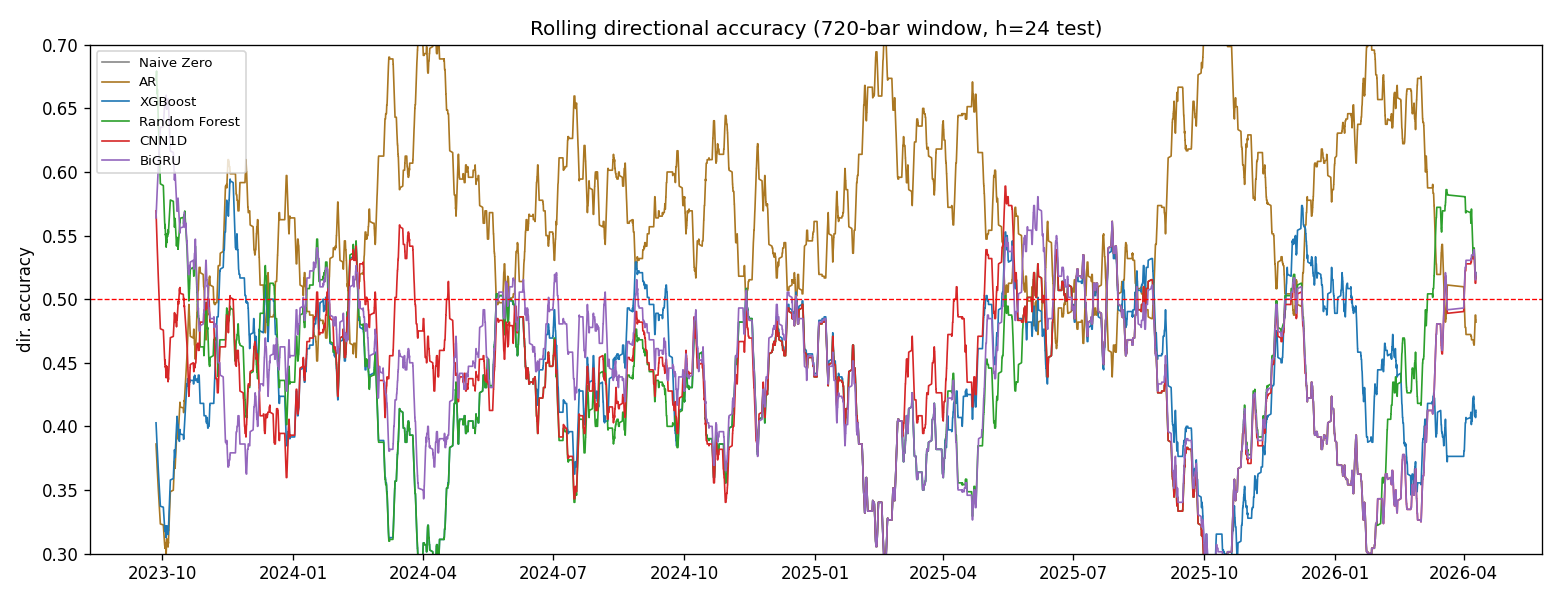
\includegraphics[width=\linewidth]{comparison/cmp_h24_rolling_diracc.png}
\caption{Précision directionnelle glissante (fenêtre 720 bougies) — test h=24.}
\end{figure}
\noindent\textbf{Interprétation.} Les courbes oscillent autour de 0,5 et se
croisent fréquemment : aucun modèle ne domine de manière persistante dans le temps,
illustrant l'instabilité du signal directionnel à cet horizon.

\begin{figure}[H]
\centering
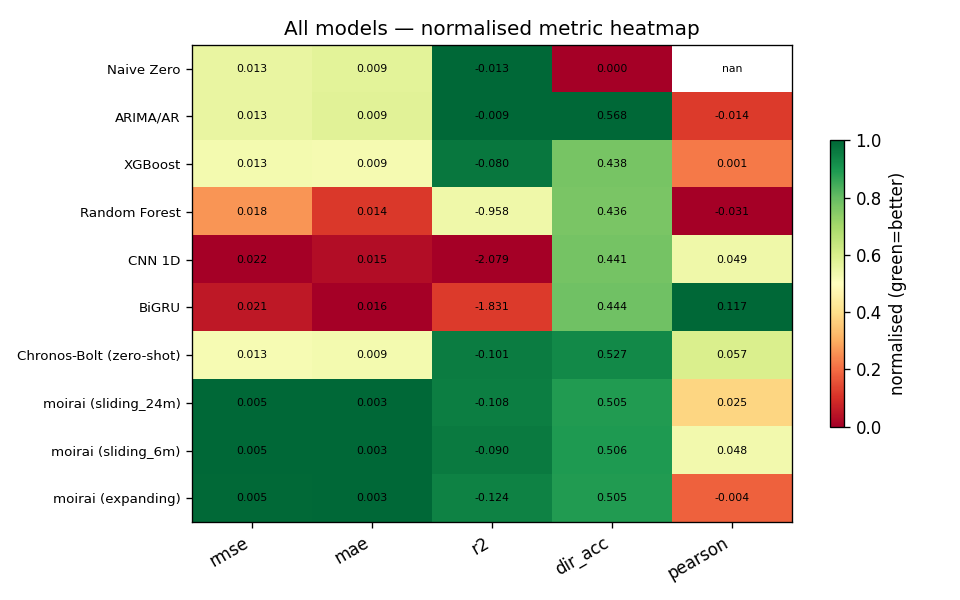
\includegraphics[width=0.8\linewidth]{comparison/cmp_metric_heatmap.png}
\caption{Heatmap normalisée des métriques (vert = meilleur) — tous modèles.}
\end{figure}
\noindent\textbf{Interprétation.} La heatmap synthétise le verdict : les lignes
« vertes » (bonnes) correspondent aux baselines et aux TSFMs ; les modèles
entraînés en interne sont majoritairement « rouges » sur le test.

% =====================================================================
\section{Phase 5 — Walk-forward et horizon court (h=4)}
% =====================================================================

\begin{figure}[H]
\centering
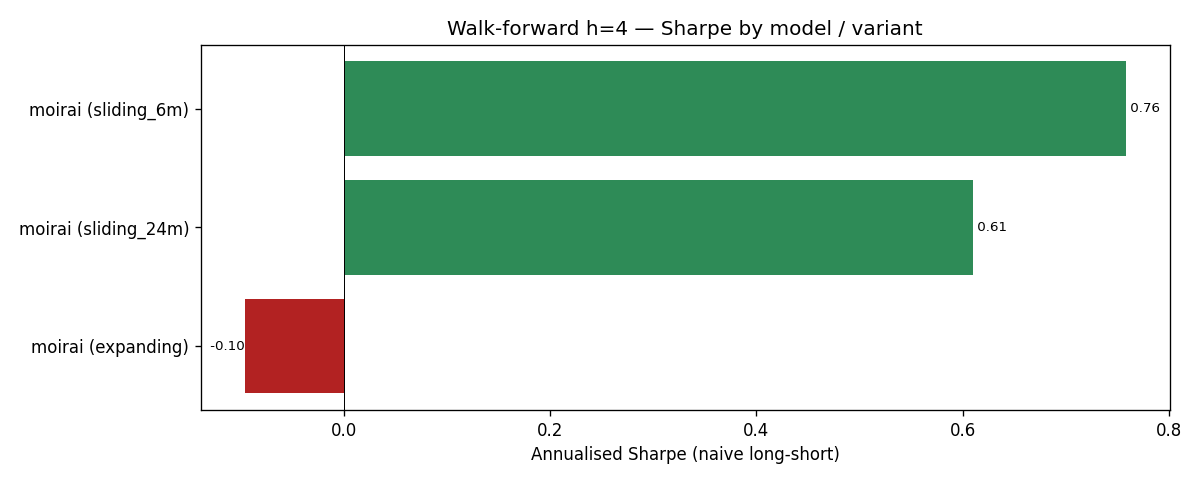
\includegraphics[width=0.7\linewidth]{final/final_sharpe_walkforward.png}
\caption{Ratio de Sharpe annualisé par modèle/variante — walk-forward h=4.}
\end{figure}
\noindent\textbf{Interprétation.} Avec un horizon court (4h) et un protocole
walk-forward (réentraînement glissant), un signal positif émerge enfin. Le modèle
champion \textbf{MOIRAI en fenêtre glissante 6 mois} atteint un Sharpe annualisé de
$\approx 0.76$. Les modèles à arbres (XGBoost) restent globalement négatifs ou
faibles ; les TSFMs zero-shot dominent.

\begin{figure}[H]
\centering
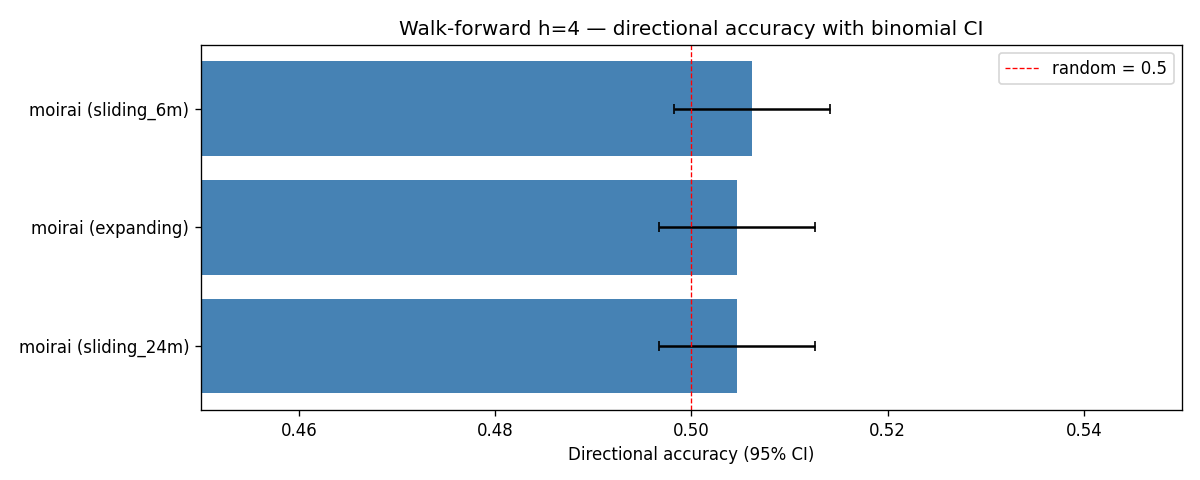
\includegraphics[width=0.7\linewidth]{final/final_diracc_ci.png}
\caption{Précision directionnelle avec intervalle de confiance binomial à 95\,\% — walk-forward h=4.}
\end{figure}
\noindent\textbf{Interprétation.} Les précisions directionnelles se situent entre
0,49 et 0,51. Les intervalles de confiance recoupent 0,5 pour la plupart : la
précision directionnelle \emph{seule} n'est pas statistiquement significative
(test binomial $p\approx 0.12$ pour le champion). Le gain de Sharpe provient donc
d'un signal \emph{pondéré par l'amplitude} (le modèle vise mieux les gros
mouvements) plutôt que d'une simple amélioration du taux de bonnes directions.

\begin{figure}[H]
\centering
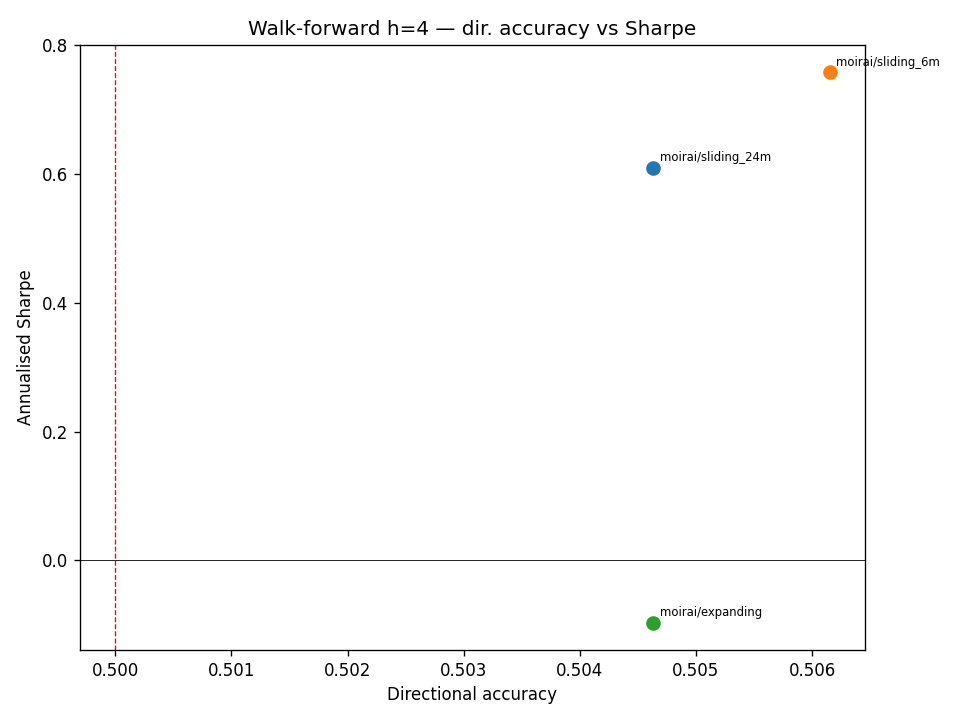
\includegraphics[width=0.65\linewidth]{comparison/cmp_wf_diracc_vs_sharpe.png}
\caption{Précision directionnelle vs Sharpe — walk-forward h=4.}
\end{figure}
\noindent\textbf{Interprétation.} Le nuage met en évidence que des modèles à
précision directionnelle quasi identique ($\approx 0.505$) peuvent avoir des Sharpe
très différents : la qualité des prédictions sur les mouvements de forte amplitude
prime. MOIRAI (sliding 6m) se détache en haut.

\begin{figure}[H]
\centering
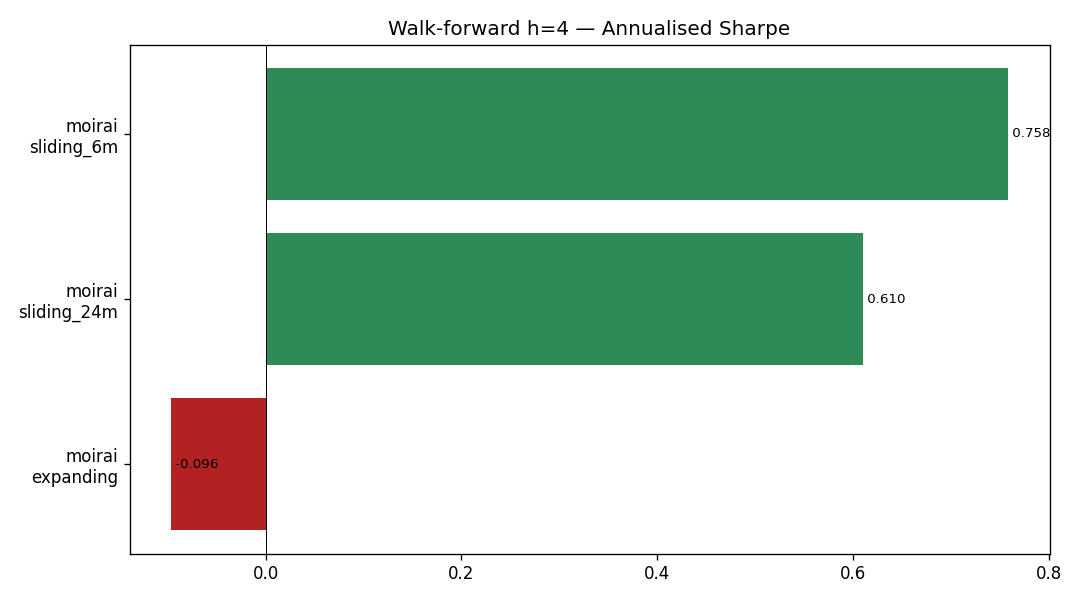
\includegraphics[width=0.49\linewidth]{comparison/cmp_wf_sharpe.png}
\hfill
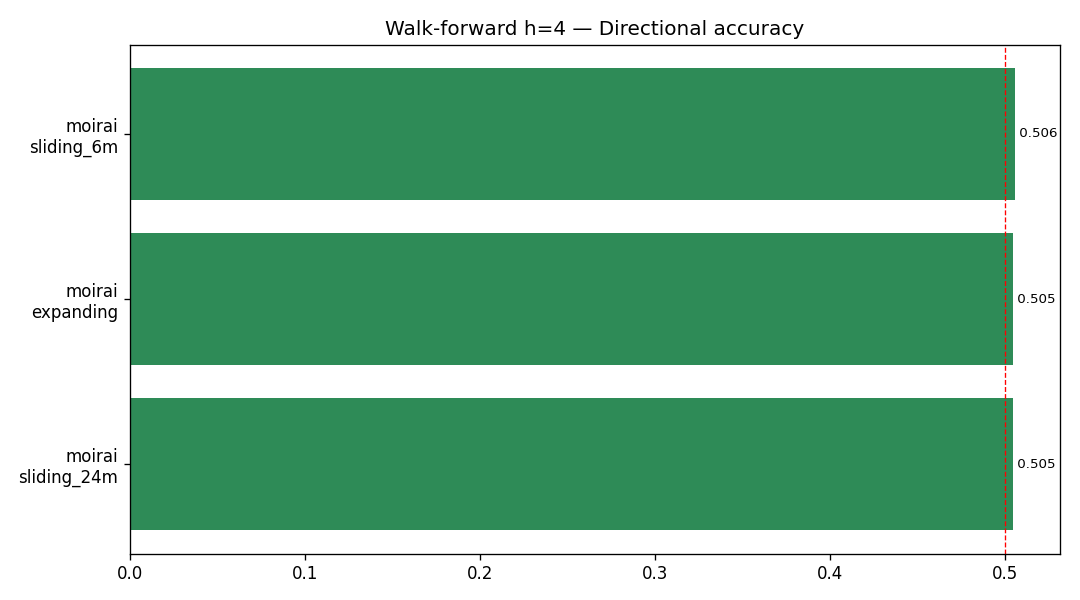
\includegraphics[width=0.49\linewidth]{comparison/cmp_wf_dir_acc.png}
\caption{Sharpe (gauche) et précision directionnelle (droite) — walk-forward, toutes variantes.}
\end{figure}
\noindent\textbf{Interprétation.} Comparaison des variantes de fenêtrage. Pour
MOIRAI, la fenêtre glissante courte (6 mois) maximise le Sharpe, alors que la
fenêtre expansive (tout l'historique) le dégrade : rester « dans le régime »
courant est bénéfique pour ce TSFM. Pour XGBoost, c'est l'inverse — l'expanding est
le moins mauvais — ce qui souligne que la stratégie de fenêtrage optimale dépend du
modèle.

\paragraph{Diagnostics détaillés du champion (MOIRAI, sliding 6m).}
\begin{figure}[H]
\centering
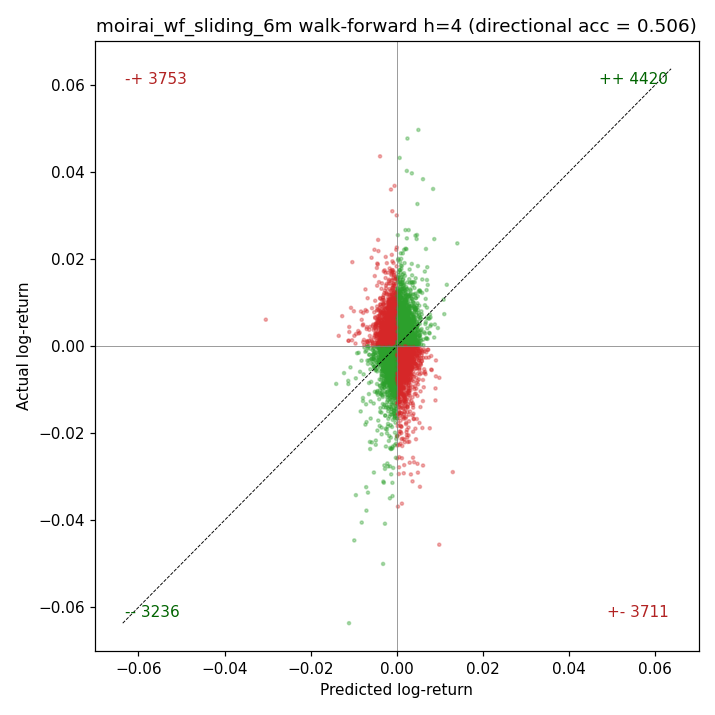
\includegraphics[width=0.49\linewidth]{walkforward/moirai_wf_sliding_6m_h4_returns.png}
\hfill
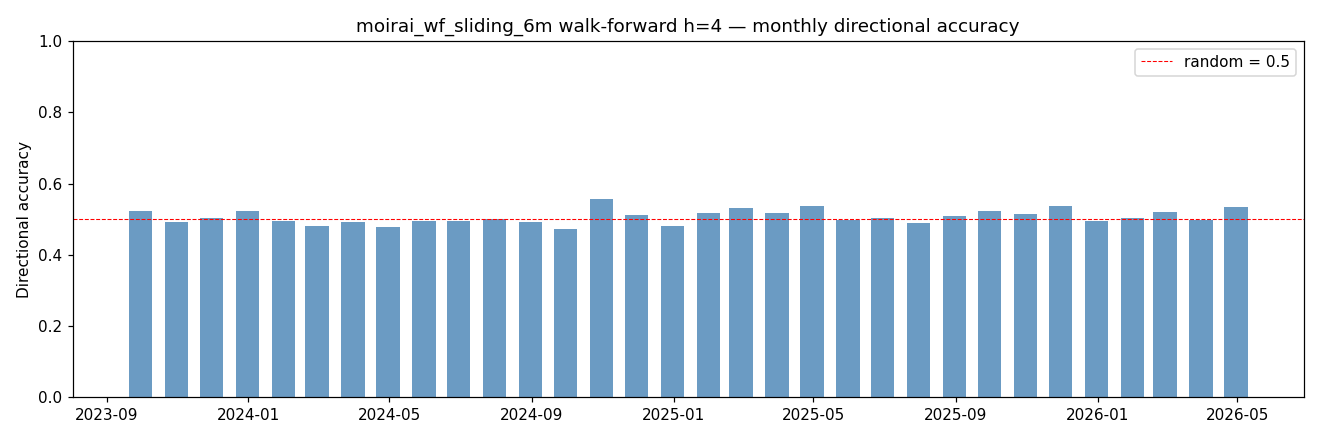
\includegraphics[width=0.49\linewidth]{walkforward/moirai_wf_sliding_6m_h4_monthly_diracc.png}
\caption{Nuage rendement prédit/réel avec quadrants (gauche) et précision directionnelle mensuelle (droite) — MOIRAI champion.}
\end{figure}
\noindent\textbf{Interprétation.} Le nuage des rendements montre une légère
prédominance des quadrants « bonne direction » (vert). La précision mensuelle est
majoritairement au-dessus de 0,5 sur la période de test, avec des mois plus
favorables que d'autres — la performance n'est pas uniforme dans le temps mais
reste globalement positive.

\begin{figure}[H]
\centering
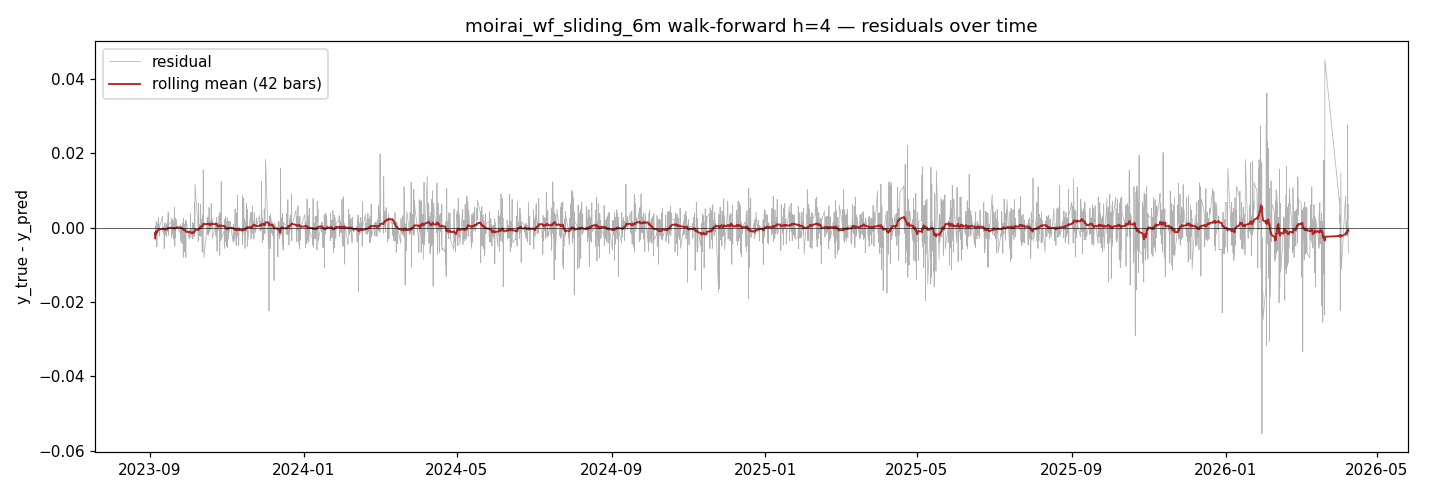
\includegraphics[width=0.49\linewidth]{walkforward/moirai_wf_sliding_6m_h4_residuals_ts.png}
\hfill
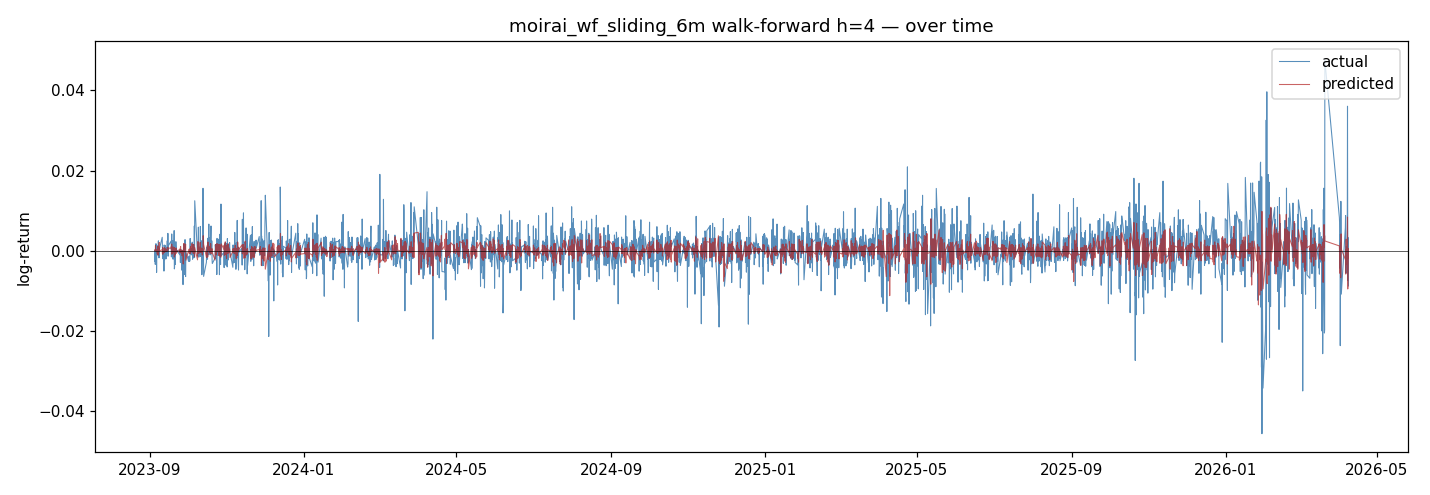
\includegraphics[width=0.49\linewidth]{walkforward/moirai_wf_sliding_6m_h4_ts.png}
\caption{Résidus dans le temps (gauche) et prédiction vs réel (droite) — MOIRAI champion.}
\end{figure}
\noindent\textbf{Interprétation.} Contrairement aux modèles entraînés, les résidus
de MOIRAI ne présentent pas de dérive systématique (biais $\approx 0$) : le
foundation model reste calibré sur toute la période de test, sans surapprentissage
d'un régime particulier.

% =====================================================================
\section{Synthèse}
% =====================================================================
\noindent
Les figures convergent vers trois conclusions robustes :
\begin{enumerate}
  \item \textbf{À horizon 24h, la prédiction du rendement est hors de portée}
        (tous $R^2$ négatifs, corrélations nulles) — cohérent avec l'efficience
        faible du marché de l'or.
  \item \textbf{La complexité du modèle aggrave le surapprentissage} face au
        régime shift 2023--2026 : Naïve $>$ XGBoost $>$ RF $>$ BiGRU $>$ CNN.
  \item \textbf{À horizon court (4h) avec walk-forward, un signal exploitable
        émerge}, capté principalement par les Time Series Foundation Models
        (MOIRAI, Chronos) grâce à leur pré-entraînement cross-domaine. Le champion
        MOIRAI atteint un Sharpe de $0.76$, à interpréter comme un signal
        \emph{directionnel pondéré par l'amplitude}, non comme une précision
        directionnelle significative.
\end{enumerate}

\end{document}
